\documentclass[a4paper,12pt,titlepage]{article}

\usepackage[a4paper]{geometry}

% \setlength{\paperheight}{297mm} 
% \setlength{\paperwidth}{210mm}
 \setlength{\textheight}{252mm} 
 \setlength{\textwidth}{160mm}
 \setlength{\hoffset}{-4mm} 
 \setlength{\voffset}{-9mm}
% \setlength{\oddsidemargin}{0mm} 
% \setlength{\topmargin}{0mm}
% \setlength{\headheight}{0mm} 
% \setlength{\headsep}{0mm}
% \setlength{\footskip}{2cm} 
% \setlength{\marginparsep}{0mm}
% \setlength{\marginparwidth}{0mm} 
\linespread{1.0}
\setlength{\parskip}{4pt plus 1pt minus .5pt}
\setlength{\parindent}{7mm} 

\renewcommand\tablename{\textbf{Table}}
\renewcommand\figurename{\textbf{Figure}} 
%\renewcommand\subsubsection{\large \textit \normalsize}

\setcounter{tocdepth}{4}

\usepackage{epsfig}
\usepackage{amsfonts} 
\usepackage{amssymb} 
\usepackage{hyperref}
\usepackage{caption}
\usepackage{verbatim}
\usepackage{setspace} % added by clangini to set single spacing for fig. captions
\usepackage{amsmath} % added by clangini

%\voffset=-8mm
%\hoffset= 5mm
%\topmargin=0mm
%\headheight=0in
%\headsep=8mm
%\footheight=0in
%\footskip=0in
%\textheight=234mm
%\textwidth=148mm
%\oddsidemargin=0in
%\evensidemargin=0in
%\pagestyle{myheadings}
%\markboth{}{}
\usepackage{graphics}

\begin{document}
%\baselineskip=8mm

%\setcounter{page}{172}

\bibliographystyle{unsrt}

\appendix

%\hoffset= 5mm

\thispagestyle{empty}

\begin{center}

%\vspace*{1cm}

{\bf{\Huge Manual for SEED}}

{\bf a program for fragment docking with force field-based evaluation of binding energy}

\vspace{0.5cm}

{\bf{\large SEED = Solvation Energy for Exhaustive Docking}}

\vspace{1cm}

\end{center}

\vspace{2cm}
\noindent
{\bf SEED developers} \\
1998 - 2008: Nicolas Majeux, Marco Scarsi, Joannis Apostolakis, Fabian Dey, \\
\hspace*{2.2cm} Claus Ehrhardt and Amedeo Caflisch \\
2011 - 2013: Fabian Dey, Tim Knehans, Emilie Frugier and Amedeo Caflisch\\
2016 - 2017: Cassiano Langini, Jean-R\'{e}my Marchand and Amedeo Caflisch

\vspace{0.9cm}

\begin{center}
{\bf
Manual for Version 4.0

June 2017
}

\end{center}

\vspace{1cm}

\linespread{1.0}

%\begin{center}
%See also:
%\end{center}

\noindent
{\normalsize
Kindly reference the original paper if you use SEED:}

{\small
\noindent
N. Majeux, M. Scarsi, J. Apostolakis, C. Ehrhardt, and A. Caflisch.
Exhaustive docking of molecular fragments on protein binding sites 
with electrostatic solvation. \\
{\it Proteins: Structure, Function and Genetics}, 
{\bf 37}:88-105, 1999. \hspace*{1cm}
}
\href{http://www.biochem-caflisch.uzh.ch/static/pdf/majeux99.pdf}{[click here for pdf]}
%
\\[4mm]
The description of the fast energy evaluation is in the second SEED paper: \\
{\small
\noindent
N. Majeux, M. Scarsi, and A. Caflisch.
Efficient electrostatic solvation model for protein-fragment docking. \\
{\it Proteins: Structure, Function and Genetics}, 
{\bf 42}:256-268, 2001. \hspace*{1cm}
}
\href{http://www.biochem-caflisch.uzh.ch/static/pdf/majeux01.pdf}{[click here for pdf]}



\vspace{0.5cm}

%\newpage

\noindent
To improve this documentation, please send comments and feedback to: \\[-1mm]
Amedeo Caflisch,  %\\ 
caflisch@bioc.uzh.ch \\
%FAX:    (41 1) 635 68 62 \\


\linespread{1.5}

\newpage

\setcounter{page}{1}
\pagenumbering{roman}

\tableofcontents

%\newpage
%
%\setcounter{page}{1}
%\pagenumbering{roman}
%
%\begin{tabular}{llllr}
%\multicolumn{5}{l}{\Huge{\bf Contents}} \\
%\\
%\Large{\bf A} & \multicolumn{4}{l}{\large{\bf Getting started}} \\
% & A.1  & \multicolumn{2}{l}{SEED Overview}                                                  &  \hspace{3cm} 1 \\
% & A.2  & \multicolumn{2}{l}{Run SEED}                                                     &  1 \\
% & A.3  & \multicolumn{2}{l}{Files required for a SEED run}                                &  1 \\
% & A.4  & \multicolumn{2}{l}{Most frequently modified parameters}                          &  1 \\
% & A.5  & \multicolumn{2}{l}{Most important output files}                                  &  1 \\
% & A.6  & \multicolumn{2}{l}{Start a new project}                                          &  1 \\
%\Large{\bf B} & \multicolumn{4}{l}{\large{\bf Carrying on}} \\
% & B.1  & \multicolumn{2}{l}{Vectors for docking}                                          &  1 \\
% &      & B.1.1                                   & Vectors for polar docking              &  2 \\
% &      & B.1.2                                   & Vectors for apolar docking             &  2 \\
% & B.2  & \multicolumn{2}{l}{Energy in SEED}                                               &  4 \\
% &      & B.2.1                                   & Accurate model                         &  5 \\
% &      &                                         & Van der Waals interaction              &  5 \\
% &      &                                         & Partial desolvation of the receptor    &  6 \\
% &      &                                         & Screened fragment-receptor interaction &  7 \\
% &      &                                         & Partial desolvation of the fragment    &  8 \\
% &      & B.2.2                                   & Fast model                             &  5 \\
% &      &                                         & Van der Waals interaction              &  9 \\
% &      &                                         & Partial desolvation of the receptor    & 10 \\
% &      &                                         & Screened fragment-receptor interaction & 11 \\
% &      &                                         & Partial desolvation of the fragment    & 12 \\
% & B.3  & \multicolumn{2}{l}{Docking schemes}                                              & 12 \\
% &      & B.3.1                                   & Slow docking scheme                    & 12 \\
% &      & B.3.2                                   & Fast docking scheme                    & 13 \\
% &      &                                         & Clustering procedure                   & 14 \\
% &      & B.3.3                                   & Postprocess scheme                     & 15 \\
%\end{tabular}
%
%\newpage
%
%\begin{tabular}{llllr}
% & B.4  & \multicolumn{2}{l}{Energy evaluation mode}                                       & \hspace{6.4cm} 15 \\
% & B.5  & \multicolumn{2}{l}{SEED output files}                                            & 15 \\
% &      & B.5.1                                   & Slow docking scheme                    & 15 \\
% &      & B.5.2                                   & Fast docking scheme                    & 16 \\
% &      & B.5.3                                   & Postprocess scheme                     & 16 \\
%\end{tabular}

\newpage

\setcounter{page}{1}
\pagenumbering{arabic}

\section{Getting started}

\subsection{Aim of SEED}

The docking approach implemented in the program SEED~\cite{Majeux:Exhaustive,Majeux:Efficient} 
determines optimal positions and orientations 
of small-to-medium-sized molecular fragments in the binding site of a rigid protein 
(hereafter also referred to as receptor) and ranks them 
according to their binding energy. Polar fragments are positioned such that 
at least one hydrogen bond with optimal distance to a protein polar group is made (polar docking). 
For the docking of apolar fragments a novel procedure has been developed to select 
in an accurate and efficient way the hydrophobic regions of 
the protein, i.e., those with low electrostatic desolvation and favorable 
van der Waals interactions with an uncharged probe sphere. 
Furthermore, the numerical Generalized Born methodology developed in the Caflisch group 
{\cite{Scarsi:Continuum,Scarsi:Comparison}} and {\it ad hoc} look-up tables are 
employed to efficiently evaluate the protein and fragment desolvation 
upon binding and the screened electrostatic interaction. 

\subsection{Running SEED}

The command to run SEED in a Unix shell is

{\tt seed.exe seed.inp >\& seed.log}

\noindent
where {\tt seed.exe} and {\tt seed.inp} are the executable and the input file, respectively.

\subsection{Files required for a SEED run}

The files required for a SEED run are:

\begin{itemize}

\item
The file {\tt seed.inp} contains the most frequently modified input values.

\item
The parameter file {\tt seed.par} contains less frequently modified input/output options, parameters for docking, energy and clustering.

The two files {\tt seed.inp} and {\tt seed.par} have comment lines which start with a \# and both files 
terminate with the word {\tt end}. All the other lines are information read by the program. In the following, 
lines referring to the input (see page 6) and parameter 
(see pages 23-26) files are indicated by {\bf i} and {\bf p}, respectively. Please note that the values shown are only indicative. For a working example refer to the test cases provided with the distribution.

The path for the parameter file is in the first line of the input file (referred to as {\bf i1}).

\item
A standard SYBYL mol2 format file containing all the fragments to dock (\textbf{i7}).
This file is simply the concatenation of all the fragments, expressed in mol2 format. Note that different conformations of the same fragment are treated as different fragments.
Partial charges are written in the 9th column in the \texttt{@$<$TRIPOS$>$ATOM} record as for the receptor.\\
In order to assign the correct Van der Waals parameters from the file \texttt{seed.par}, the CHARMM atom types should be specified in the mol2 file. This is done using the alternative atom type specified by the record \texttt{@<TRIPOS>ALT\_TYPE}, which takes the following form:
\begin{verbatim}
@<TRIPOS>ALT_TYPE
CGenFF_4.0_ALT_TYPE_SET
CGenFF_4.0 1 CG331 2 CG301 3 CG331 4 CG324 ...
\end{verbatim}
Where \texttt{CGenFF\_4.0\_ALT\_TYPE\_SET} sets a user-defined name (for example \texttt{CGenFF\_4.0}) for the alternative atom type set. This name is repeated on the next line, followed by the list of atom number-atom type pairs for each atom in the molecule. This list should span a single line, but can be broken by using \texttt{\textbackslash\textbackslash}.\\
%It is recommended to keep the SYBYL atom types on the 6th column of the record \texttt{@$<$TRIPOS$>$ATOM} as they are recognized by most cheminformatics and visualization software.\\
The first line of the SYBYL record \texttt{@$<$TRIPOS$>$MOLECULE} specifies the fragment name. It is convenient (but not necessary) to have unique names for each fragment. In case fragments with duplicate names are found in the input, they will be renamed in all the output files appending to their name the dollar sign \$ and an incremental index.
As the fragment mol2 input file is read sequentially, the number of fragments in it does not have to be specified a priori.

\item
A standard SYBYL mol2 file ({\bf i2}) for the receptor with partial charges on the 
9th column in the {\tt @$<$TRIPOS$>$ATOM} record and CHARMM atom types specified by the {\tt @$<$TRIPOS$>$ALT\_TYPE} record (refer to the fragment file description for details).

\end{itemize}

\subsection{Input file parameters}

In the following, parameters of the input file {\tt seed.inp} (page 6) 
are explained.

\noindent
{\bf i1}
Path for the parameter file {\tt seed.par}.

\noindent
{\bf i2}
Receptor coordinate file (SYBYL mol2 format).

\noindent
{\bf i3}
The first line is the number of residues in the binding site and the 
following lines are the residue sequential numbers 
(e.g. if Arg\_38 is the first residue of the protein, its sequential 
number is 1 and not 38). Binding site metal ions 
have to be in the list.

\noindent
{\bf i4}
The first line is the number of user-selected points in the binding site and 
the following lines are their coordinates. These points are used to select 
polar and apolar receptor vectors that meet an angle criterion 
({\bf p14}, see \ref{sssec:select}) such that vectors pointing outside of the binding site 
are discarded. The points can be for example the fragment heavy atoms of 
a known fragment-receptor complex structure. 

\noindent
\textbf{i5}
The first line is the total number of vectors (refer to \ref{ssec:VecDock} for their meaning) for the 
metal ions and each of the following lines contains the atom index of the metal as it is in 
the receptor mol2 file and the coordinates of the vector extremity.

\noindent
{\bf i6}
Coordinates of the center and radius of the sphere in which the geometry center of 
the fragment position must be to be accepted. This filter can be discarded by selecting 
{\tt n} instead of {\tt y}.

\noindent
\textbf{i7}
First line: a character specifying the computation mode: \texttt{e} if energy evaluation only
has to be carried out (see \ref{ssec:Energy}) or \texttt{d} if docking is 
also requested (see \ref{ssec:Docking}).
Following line: the first column contains the path of the fragment mol2 file and the 
second column allows the selection of apolar, polar docking or both. 
The fragment position is accepted if the total energy (according to the approximate model of section \ref{fast:model}) is smaller than a cutoff 
given in the third column. The second clustering (see \ref{par:Clustering}) is applied on the positions 
for which the binding energy of the cluster representative is smaller than a cutoff 
value specified in the 4th column.






% \noindent
% {\bf i2}
% Dielectric constant of the solute (receptor and fragment), usually between 1.0 
% and 4.0.

% \noindent
% {\bf i4}
% Number of cluster members saved in output files and postprocessed 
% with the more accurate solvation model (see \ref{sssec:Post}).

% \noindent
% {\bf i13}
% First line: the integer is the number of fragment files. The second term can be set to {\tt y} 
% (energy evaluation mode; see \ref{ssec:Energy}) or to {\tt n} (docking mode; see \ref{ssec:Docking}). 
% Following lines: the first column contains the 
% path of the mol2 file and the second column allows the selection of apolar, polar docking or 
% both. The fragment position is accepted if the total energy is smaller than a cutoff given 
% in the third column. The second clustering (see page \pageref{par:Clustering}) is applied on the 
% positions for which the binding 
% energy of the cluster representative is smaller than a cutoff value specified in the 4th column. 


\subsection{Most important output files}
\label{ssec:MostOut}

The main output file, whose filename is specified in {\bf p6}, contains the energy 
values and results of clustering.

\noindent
A directory {\tt outputs} in which all the output files are written is 
automatically created by the program. Note that if a directory named \texttt{outputs} is
already present, it will be overwritten by the SEED run.

\noindent
{\tt $<$FragmentMol2FileName$>$\_clus.mol2} contains the fragment positions with 
best energy after the postprocessing step. This file is the concatenation of a mol2 file 
for each saved pose. The maximum number of poses to be saved per cluster can be set in 
\textbf{p5} (first value). The comment line of the SYBYL mol2 record \texttt{@$<$TRIPOS$>$MOLECULE} (6th 
line after the record identifier) contains some useful information about the pose,
\textit{i.e.} increasing pose index, cluster number, total energy and fragment number
(\texttt{Fr\_nu}). The latter represents the program internal numbering of the pose and it is not interesting \textit{per se}, but it can be used to match the pose to docking information written in the main output file.

\noindent
\texttt{seed\_clus.dat} is a summary table containing the separate energy terms for each fragment position saved to {\tt $<$FragmentMol2FileName$>$\_clus.mol2}. This information can be also retrieved from the main output file. Columns are organized as follows:
\begin{enumerate}
\item \textbf{Name:} Fragment name.
\item \textbf{Pose:} Incremental pose number. This index restarts at 1 for each new fragment.
\item \textbf{Cluster:} Cluster number.
\item \textbf{Fr\_nu:} Fragment number. This is SEED internal pose number.
\item \textbf{Tot:} Total binding energy.
\item \textbf{ElinW:} Electrostatic interaction in water.
\item \textbf{rec\_des:} Desolvation of the receptor upon complex formation.
\item \textbf{frg\_des:} Desolvation of the fragment upon complex formation.
\item \textbf{vdW:} Van der Waals interaction energy.
\item \textbf{DElec:} Electrostatic difference upon fragment binding. It is given by $ElinW-DG\_hydr$. It roughly represents how good the fragment feels in the protein compared to how good it feels in water. 
\item \textbf{DG\_hydr:} Free energy of hydration of the fragment.
\item \textbf{Tot\_eff:} $Tot/HAC$.
\item \textbf{vdW\_eff:} $vdW/HAC$
\item \textbf{Elec\_eff:} $ElinW/HAC$ 
\item \textbf{HAC:} Heavy atom count. It is the total number of non-hydrogen atoms in the fragment.
\item \textbf{MW:} Molecular weight of the fragment.
\end{enumerate}

\noindent
{\tt $<$FragmentMol2FileName$>$\_best.mol2} contains the best fragment positions, according to the total energy, irrespective of the cluster they belong to (parameter \textbf{p5}, second value). The difference with respect to {\tt $<$FragmentMol2FileName$>$\_clus.mol2} is that the user can set the total number of poses to be saved instead of the number of cluster members.

\noindent
\texttt{seed\_best.dat} is the same as \texttt{seed\_clus.dat} but matching \\{\tt $<$FragmentMol2FileName$>$\_best.mol2}.

\noindent
Note that the number of cluster members to be saved (first value of \textbf{p5}) determines 
the maximum number of poses for which to evaluate the slow energy during postprocessing. Thus 
in general it is advisable to set this number to a value higher than one, in order to be sure to consider a meaningful number of poses, and to suppress the corresponding mol2 file output (first value of \textbf{p3} set to no) as it may quickly become big.

\subsection{Starting a new project}

When a new project is started, it is useful to first generate the vectors 
without docking any fragment ({\bf i7} set to {\tt d}). 
Of the six files listed below one should visualize the two files 
{\tt polar\_rec\_reduc.mol2} and {\tt apolar\_rec\_reduc.mol2}. It is 
useful to modify the appropriate parameters 
if the vector distributions do not meet the user's expectation, since 
fragments are docked using the vectors present in the two aforementioned 
files. After this test one has just to read the maps ({\bf p7-p8}: {\tt r}) 
instead of generating them again.

\begin{itemize}

\item
{\tt polar\_rec.mol2} contains vectors distributed uniformly on a spherical region 
around each ideal H-bond direction. The deviation from ideal hydrogen bond geometry 
and the number of additional vectors to distribute uniformly on the spherical region 
are set in {\bf p12}.

\item
{\tt polar\_rec\_reduc\_angle.mol2} contains vectors of {\tt polar\_rec.mol2} which 
are selected according to an angle criterion ({\bf i4}, {\bf p14}). Vectors pointing 
outside of the binding site are discarded. The file {\tt polar\_rec\_reduc\_angle.mol2} 
exists only if the angle criterion has been activated by the user ({\bf i4}).

\item
{\tt polar\_rec\_reduc.mol2} contains vectors of {\tt polar\_rec.mol2} 

\vspace{-0.2cm}
(or of {\tt polar\_rec\_reduc\_angle.mol2} if the angle criterion has been activated ({\bf i4})) 
which are selected according to favorable 
van der Waals interaction between all the receptor atoms and a spherical probe 
on the vector extremity. The aim is to discard receptor vectors that 
point into region of space occupied by other atoms of the receptor and select 
preferentially vectors in the concave regions of the receptor. The van der Waals 
radius of the probe is specified in {\bf p15}. The number of selected 
vectors is controlled with {\bf p2}. 
%The maximal number of selected 
%vectors is set in {\bf i3}. 
\item
{\tt apolar\_rec.mol2} contains points distributed uniformly on the solvent-accessible 
surface of the receptor. The density of surface points is set in {\bf p22}.

\item
{\tt apolar\_rec\_reduc\_angle.mol2} contains vectors of {\tt apolar\_rec.mol2} which 
are selected according to an angle criterion ({\bf i4}, {\bf p14}). Vectors pointing 
outside of the binding site are discarded. The file {\tt apolar\_rec\_reduc\_angle.mol2} 
exists only if the angle criterion has been activated by the user ({\bf i4}).

\item
{\tt apolar\_rec\_reduc.mol2} contains points of {\tt apolar\_rec.mol2} 

\vspace{-0.2cm}
(or of {\tt apolar\_rec\_reduc\_angle.mol2} if the angle criterion has been activated ({\bf i4})) 
which are selected 
according to their hydrophobicity. For this purpose a low dielectric sphere is placed on 
each of these points. The hydrophobicity is defined as the weighted sum of the receptor desolvation 
energy due to the presence of the probe and the probe/receptor van der Waals interaction. 
The weighting factors and the probe radius are set in {\bf p22}. The number of 
selected apolar points is controlled with {\bf p2}.

%The maximal number of 
%selected apolar points is set in {\bf i3}.

\end{itemize}

\subsection{Troubleshooting in case of empty output}

If after starting a SEED run the program exits unexpectedly, the keyword {\tt WARNING} should be 
looked for in the main output file ({\bf p6}) to find an hint on possible problems (wrong path for filenames, 
unknown value for some parameters ...).

\noindent
If the main output file does not contain any fragment position for a given fragment type, it can 
be due to several reasons: the center of the sphere ({\bf i6}) might be misplaced 
(outside the binding site), the checking of clashes ({\bf p10}, see \ref{sssec:accurdock}; 
{\bf p11}, see \ref{sssec:fastdock} and \ref{sssec:Post}) too strict, 
the van der Waals energy cutoff ({\bf p23}) for apolar fragments too severe, 
the total energy cutoff (third column of {\bf i7}) too stringent. 
To find out what the reason could be, the following part of the main output file should 
be investigated:

\vspace{0.5cm}

\begin{tabular}{l}
{\tt Total number of generated fragments of type 1 (BENZ) : 118800} \\%[-3mm]
{\tt Fragments that passed the sphere checking : 102894} \\%[-3mm]
{\tt Fragments that passed the bump checking : 49007} \\%[-3mm]
{\tt Fragments that passed the vdW energy cutoff : 22100} \\%[-3mm]
{\tt Fragments that passed the total energy cutoff : 17794}
\end{tabular}

\begin{figure}[p]
  %\centering
   \makebox[\textwidth][c]{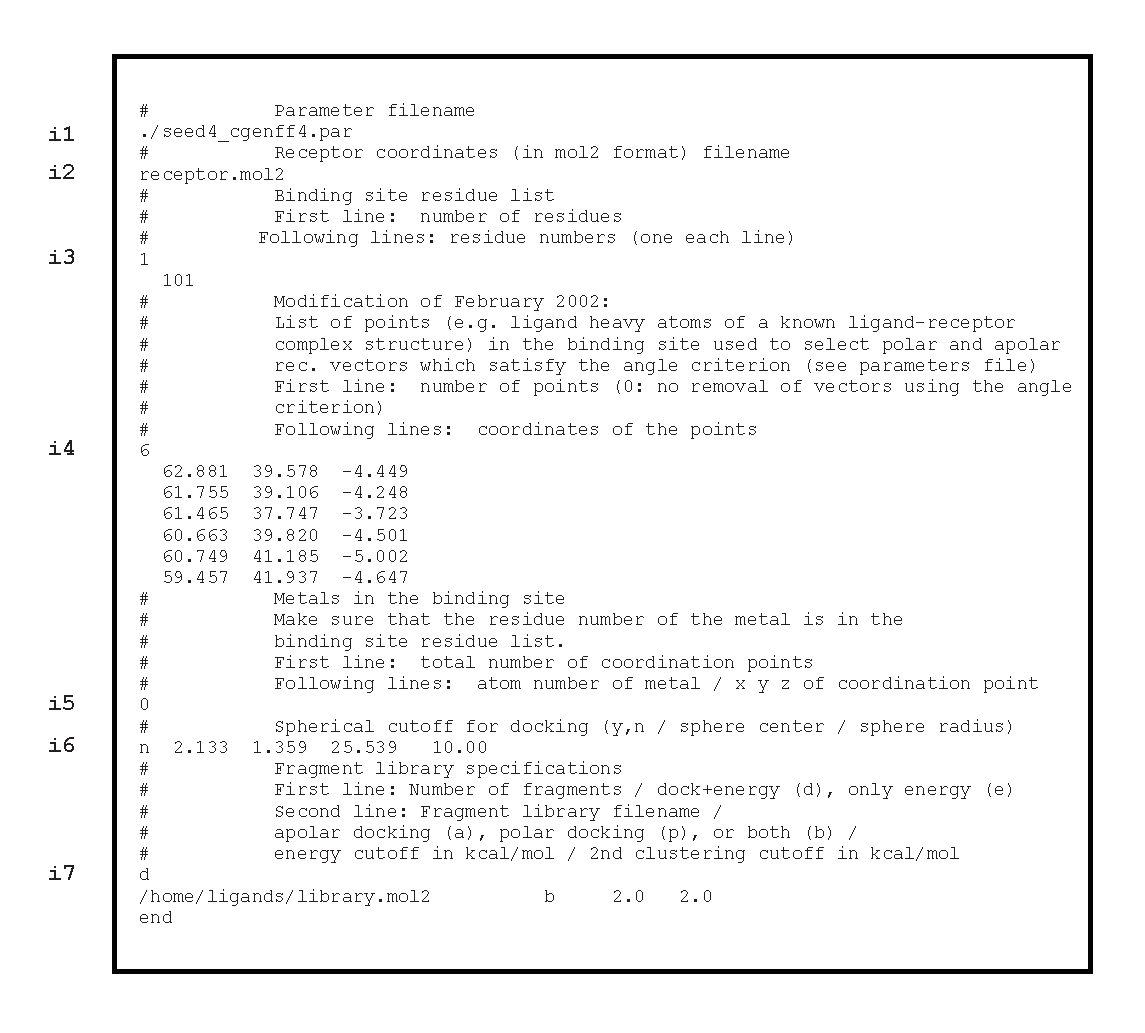
\includegraphics[width=1.2\textwidth]{data/seed_inp_final.pdf}}
  \caption{\textit{Seed input file (\textbf{seed.inp}).}}
\end{figure}

%\newpage

%\section*{}
%\addcontentsline{toc}{figure}{Input file}

%%\begin{figure}
%\vspace*{-1.7cm}
%\begin{center}
%\includegraphics[scale=0.9]{data/inp.pdf}
%\end{center}
%%\end{figure} 


\newpage

\section{Carrying on}

\subsection{Vectors for docking}
\label{ssec:VecDock}

The binding site where the fragments are to be docked is defined by a list of receptor 
residues (possibly including explicit water molecules, treated as part of the receptor 
molecule).
The first line of {\bf i3} is the number of residues in the binding site and the following lines are 
the residue sequential numbers (e.g. if Arg\_38 is the first residue of the protein, its sequential 
number is 1 and not 38). If a metal ion belongs to the binding site, its sequential number also has to be 
in the list.

\subsubsection{Vectors for polar docking}

Fragments are considered polar if they have at least one H-bond donor or acceptor. SEED docks polar 
fragments where at least one hydrogen bond with good geometry is made. 
\begin{figure}[h]
\begin{center}
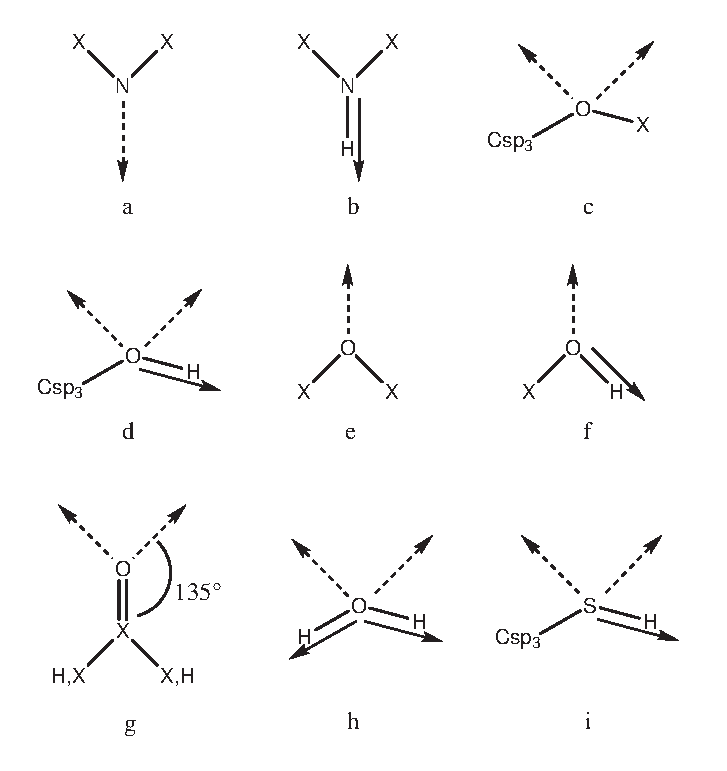
\includegraphics[scale=0.7]{figures/fig1.ps}
\end{center}
\caption{\it
Description of polar vectors for the fragment and for the receptor. X is a 
heavy atom. The broken arrow represents a vector of H-bond acceptor in the 
lone pair direction and the full arrow a vector of H-bond donor. 
The geometry of c, d, h and i is tetrahedral (angle of $109^\circ$). 
Examples: (a) imidazole, pyridine, (b) protein backbone, imidazole, indole, 
(c) ethers, (d) Ser and Thr side chains, sugars, (e) methoxybenzene, (f) Tyr side 
chain, phenol, (g) Asn, Gln, Asp, and Glu side chains, protein backbone, 
acetamide, (h) water, (i) Cys side chain.
}
\end{figure} 
First, predefined rules (Figure 1) 
allow the distribution of vectors of unitary length on all H-bond groups of the fragment in a direction 
for an ideal H-bond geometry. For example, if a nitrogen atom is bound to two heavy atoms, one H-bond 
vector is generated in the direction of either the lone pair (Figure 1a) or the NH bond (Figure 1b). The 
same procedure is then used for the polar groups in the receptor binding site (backbone and side chains). 
These 
rules are based on the atomic element number. A correspondence between atom types and atomic element 
numbers has to be given in {\bf p29}: the first line is the total number of correspondences and the first 
three terms of the following lines are respectively a sequential number, the atom type and the atomic 
element number. 
Vectors for metal ions have to be provided by the user. The first line of {\bf i5} is the total number 
of vectors for the metal ions and each of the following lines contains the atom number of the metal as 
it is in the receptor mol2 file and the coordinates of the vector extremity. The vector is then built 
by joining the vector extremity to the metal ion center. 

For the receptor polar groups and metal ions an additional set of vectors is distributed uniformly on 
a spherical region around each of the ideal directions to increase the spatial sampling. The first term 
of {\bf p12} is the maximal angular deviation from ideal hydrogen bond geometry and the second term is 
the number of additional vectors to distribute uniformly on the spherical region.

To discard receptor vectors that point into a region of space occupied by other atoms of the protein 
and select preferentially vectors in the concave regions of the receptor a spherical probe is set on 
the vector extremity at a distance corresponding to the sum of the van der Waals radii of the acceptor 
or donor atom and the probe. The van der Waals radius of the probe in \AA \, is specified in {\bf p15} and 
those of the atom types are specified in the 4th column of {\bf p29}. 
The van der Waals interaction (see below) between the probe and all the receptor atoms 
is then evaluated except for the receptor hydrogen atom involved in the H-bond. The vectors which 
show less favorable van der Waals energies are discarded. 
The number of selected polar vectors is modified through the first term of {\bf p2}. 
%The maximal number of selected polar vectors 
%is the first term of {\bf i3}. 
Finally, the docking itself is achieved by matching a H-bond vector 
of the receptor with a H-bond vector of the fragment at a distance that depends on the atom types of 
donor and acceptor involved in the hydrogen bond. These bond lengths are specified in {\bf p30} 
(a default length on the first line and two blocks where lengths are set between element types and atom 
types respectively; each block starts with the number of following lines in the block). 
The fragment is then rotated around the H-bond axis to increase sampling. The number of rotations 
is set in {\bf p13}.

\subsubsection{Vectors for apolar docking}

SEED docks apolar fragments into hydrophobic regions of the receptor. First, a number of points 
are distributed uniformly on the solvent-accessible surface (SAS) of the fragment. The density of 
surface points for the fragment is set in the second term 
of {\bf p22}. Second, an automatic procedure defines the hydrophobic regions on the 
receptor. For this purpose a number of points are uniformly distributed on the SAS of the binding site 
(density of surface points for the receptor in the first term of {\bf p22}). 
A low dielectric sphere is placed on each of these points, and the receptor desolvation energy 
(see below) and the probe/receptor van der Waals interaction are evaluated. The radius of the sphere 
is the third term of {\bf p22}: a value of 1.4~\AA \, allows a finer description of the narrow pockets 
than with a value of 1.8 \AA. The points on the receptor SAS are then ranked according to the sum of 
the two energy terms weighted by scaling factors that are the last two terms
of {\bf p22}. The number of selected apolar points can be modified with the second term of {\bf p2}. 
%The maximal 
%number of selected apolar points is the second term of {\bf i3}. 
For both the fragment and the receptor, 
vectors are defined by joining each point on the SAS with the corresponding atom center. Finally, 
apolar fragments are docked by matching a vector of the fragment with a vector of the receptor at the 
optimal van der Waals distance. To improve sampling additional rotations of the fragment are performed 
around the axis joining the receptor atom and fragment atom. The number of rotations is set in 
{\bf p13}.

\subsubsection{Selection of receptor vectors using an angle criterion}
\label{sssec:select}

(Modification of February 2002)

\noindent
To discard polar and apolar receptor vectors that point outside of the binding site 
a selection using an angle criterion (Figure 2) can be activated ({\bf i4}, {\bf p14}). 

\begin{figure}[h]
\begin{center}
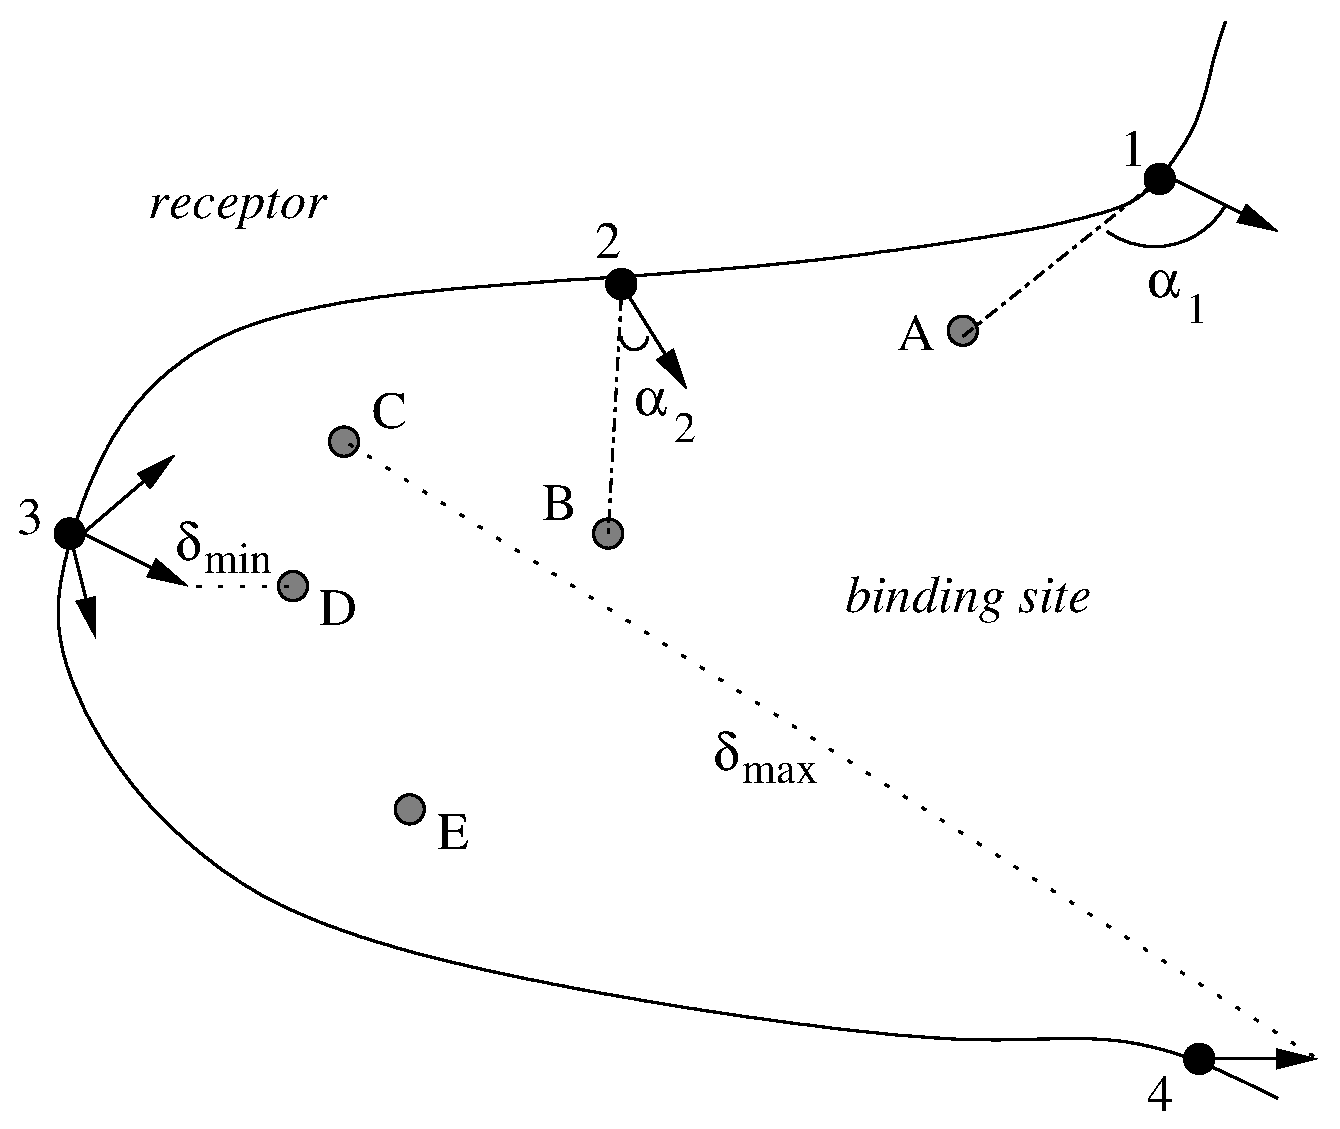
\includegraphics[scale=0.5]{figures/angle_select.eps}
\end{center}
\caption{\it
1-4: receptor atoms and vectors. A-E: user-defined anchor points in the binding site 
(e.g., fragment heavy atoms). The angle between a vector and its closest anchor point in 
the binding site is shown for two vectors ($\alpha_1$, $\alpha_2$). Reasonable 
parameters should allow to remove the vector of atom 1 from the list of receptor 
vectors and keep the vector of atom 2. 
$\delta_{min}$ and $\delta_{max}$ are defined in the text. 
}
\end{figure}

\noindent
It is applied directly after vectors have been distributed on the binding site, i.e., before the 
selection by means of a spherical probe for polar vectors and before the selection by means 
of a low dielectric sphere for apolar vectors. 
The first line of {\bf i4} is the number of user-defined anchor points in the binding site and 
the following lines are their coordinates. The anchor points can be for example the fragment heavy 
atoms obtained from a known fragment-receptor complex structure. The minimal and maximal distances 
($\delta_{min}$ and $\delta_{max}$) between the extremity of the vectors and the anchor points 
in the binding site are first evaluated. A vector is then discarded 
if the angle between the vector and the closest anchor point in the binding site 
(angle anchor\_point--vector\_origin--vector\_extremity) is larger than an angle cutoff. 
The angle cutoff is {\bf p14}$_1$ (first parameter in {\bf p14}) if the distance between the 
vector and the closest anchor point is smaller or equal to $\delta_{min} \times {\bf p14}_3$; 
the angle cutoff is {\bf p14}$_2$ if the distance is larger or equal to 
$\delta_{max} \times {\bf p14}_4$. 
For other distances the angle cutoff value falls between {\bf p14}$_1$ and 
{\bf p14}$_2$ (linear dependence). 
Reasonable parameters provide permissive angle cutoffs for vectors close to an 
anchor point and stricter angle cutoffs for distant vectors.

\subsubsection{Polar and apolar docking}

Some ``polar'' fragments can have considerable hydrophobic character (e.g., diphenyl-
ether). Therefore, 
they can also be docked by the procedure for apolar fragments. The second column of {\bf i7} allows 
the user to select apolar docking, polar docking or both.

\subsection{Energy in SEED}

The binding energy is evaluated in SEED as the sum of the Van der Waals interaction and 
the electrostatic energy.
The main assumption underlying the evaluation of the electrostatic 
energy in solution of a fragment-receptor complex is the description 
of the solvent effects by continuum electrostatics.
The system is partitioned into solvent and solute regions and 
different dielectric constants are assigned to each region 
(dielectric constant of the solute, i.e. receptor and fragment, in {\bf p1} (usually between 1.0 and 4.0) and 
dielectric constant of the solvent, normally 80 for water, as the 3rd term of {\bf p21}).
In this approximation only the intra-solute electrostatic interactions need to be evaluated explicitly, strongly reducing the number of energy evaluations with respect to an explicit treatment of the solvent. \\
The procedure to calculate the difference in electrostatic energy $\Delta G_{electr}$ upon binding of 
a fragment to a receptor is depicted in Fig. \ref{fig:thermo_cycle}. The binding process (first row of Fig. \ref{fig:thermo_cycle}) is decomposed into a cycle
by introducing an uncharged copy of the solute (white-filled receptor and fragment).
The binding free energy can then be decomposed into three terms:
\begin{itemize}
\item Partial desolvation of the receptor: electrostatic energy difference 
      upon binding an uncharged fragment to a charged receptor
      in solution.
\item Partial desolvation of the fragment: electrostatic energy difference 
      upon binding a charged fragment to an uncharged receptor in 
      solution. This term makes use of the GB treatment in the accurate energy model.
\item Screened fragment-receptor interaction: intermolecular 
      electrostatic energy in solution. This is represented as the swapping of 
      the charged and uncharged fragment in the bottom of Fig. \ref{fig:thermo_cycle}. 
      The term is written as the pairwise sum 
      $\sum_{i \in fragment, \\ j \in protein} q_i \phi_j$ 
      %\begin{equation*}
      %    \sum_{\substack{i \in fragment, \\ j \in protein}} q_i \phi_j
      %\end{equation*} 
      where the values of $\phi_j$ (i.e., the electrostatic potential of the protein atom $j$) are calculated by the GB model in the accurate energy description.
\end{itemize}
Note that the addition of the uncharged solute (highlighted 
by the brown box) does not modify the electrostatic energy as this solute 
does not interact with water.
\\
The single terms can be evaluated in SEED according to two different energy models: the accurate model (section \ref{accurate:model}) and the fast model (section \ref{fast:model}). The two models are combined together in a two-step procedure (see \ref{ssec:Docking})

%Two energy models are implemented in SEED: they can be evaluated independently or combined in a two-step 
%procedure (see \ref{ssec:Docking}). In both cases the binding energy is the sum of the van der Waals 
%interaction and the electrostatic energy. 
%The main assumption underlying the evaluation of the electrostatic 
%energy in solution of a fragment-receptor complex is the description 
%of the solvent effects by continuum electrostatics. 
%The system is partitioned into solvent and solute regions and 
%different dielectric constants are assigned to each region 
%(dielectric constant of the solute, i.e. receptor and fragment, in {\bf p1} (usually between 1.0 and 4.0) and 
%dielectric constant of the solvent, normally 80 for water, as the 3rd term of {\bf p21}).
%In this 
%approximation only the intra-solute electrostatic interactions need to 
%be evaluated. This strongly reduces 
%the number of interactions with respect to an explicit treatment of the 
%solvent.
%\begin{comment}
%The difference in electrostatic energy in solution upon binding of a 
%fragment to a receptor can be calculated as the sum of the following 
%three terms: 
%\begin{itemize}
%\item Partial desolvation of the receptor: electrostatic energy difference 
%      upon binding an uncharged fragment to a charged receptor
%      in solution.
%\item Screened fragment-receptor interaction: intermolecular 
%      electrostatic energy in solution.
%\item Partial desolvation of the fragment: electrostatic energy difference 
%      upon binding a charged fragment to an uncharged receptor in 
%      solution.
%\end{itemize}
%\end{comment}

\begin{figure}
%\begin{center}
%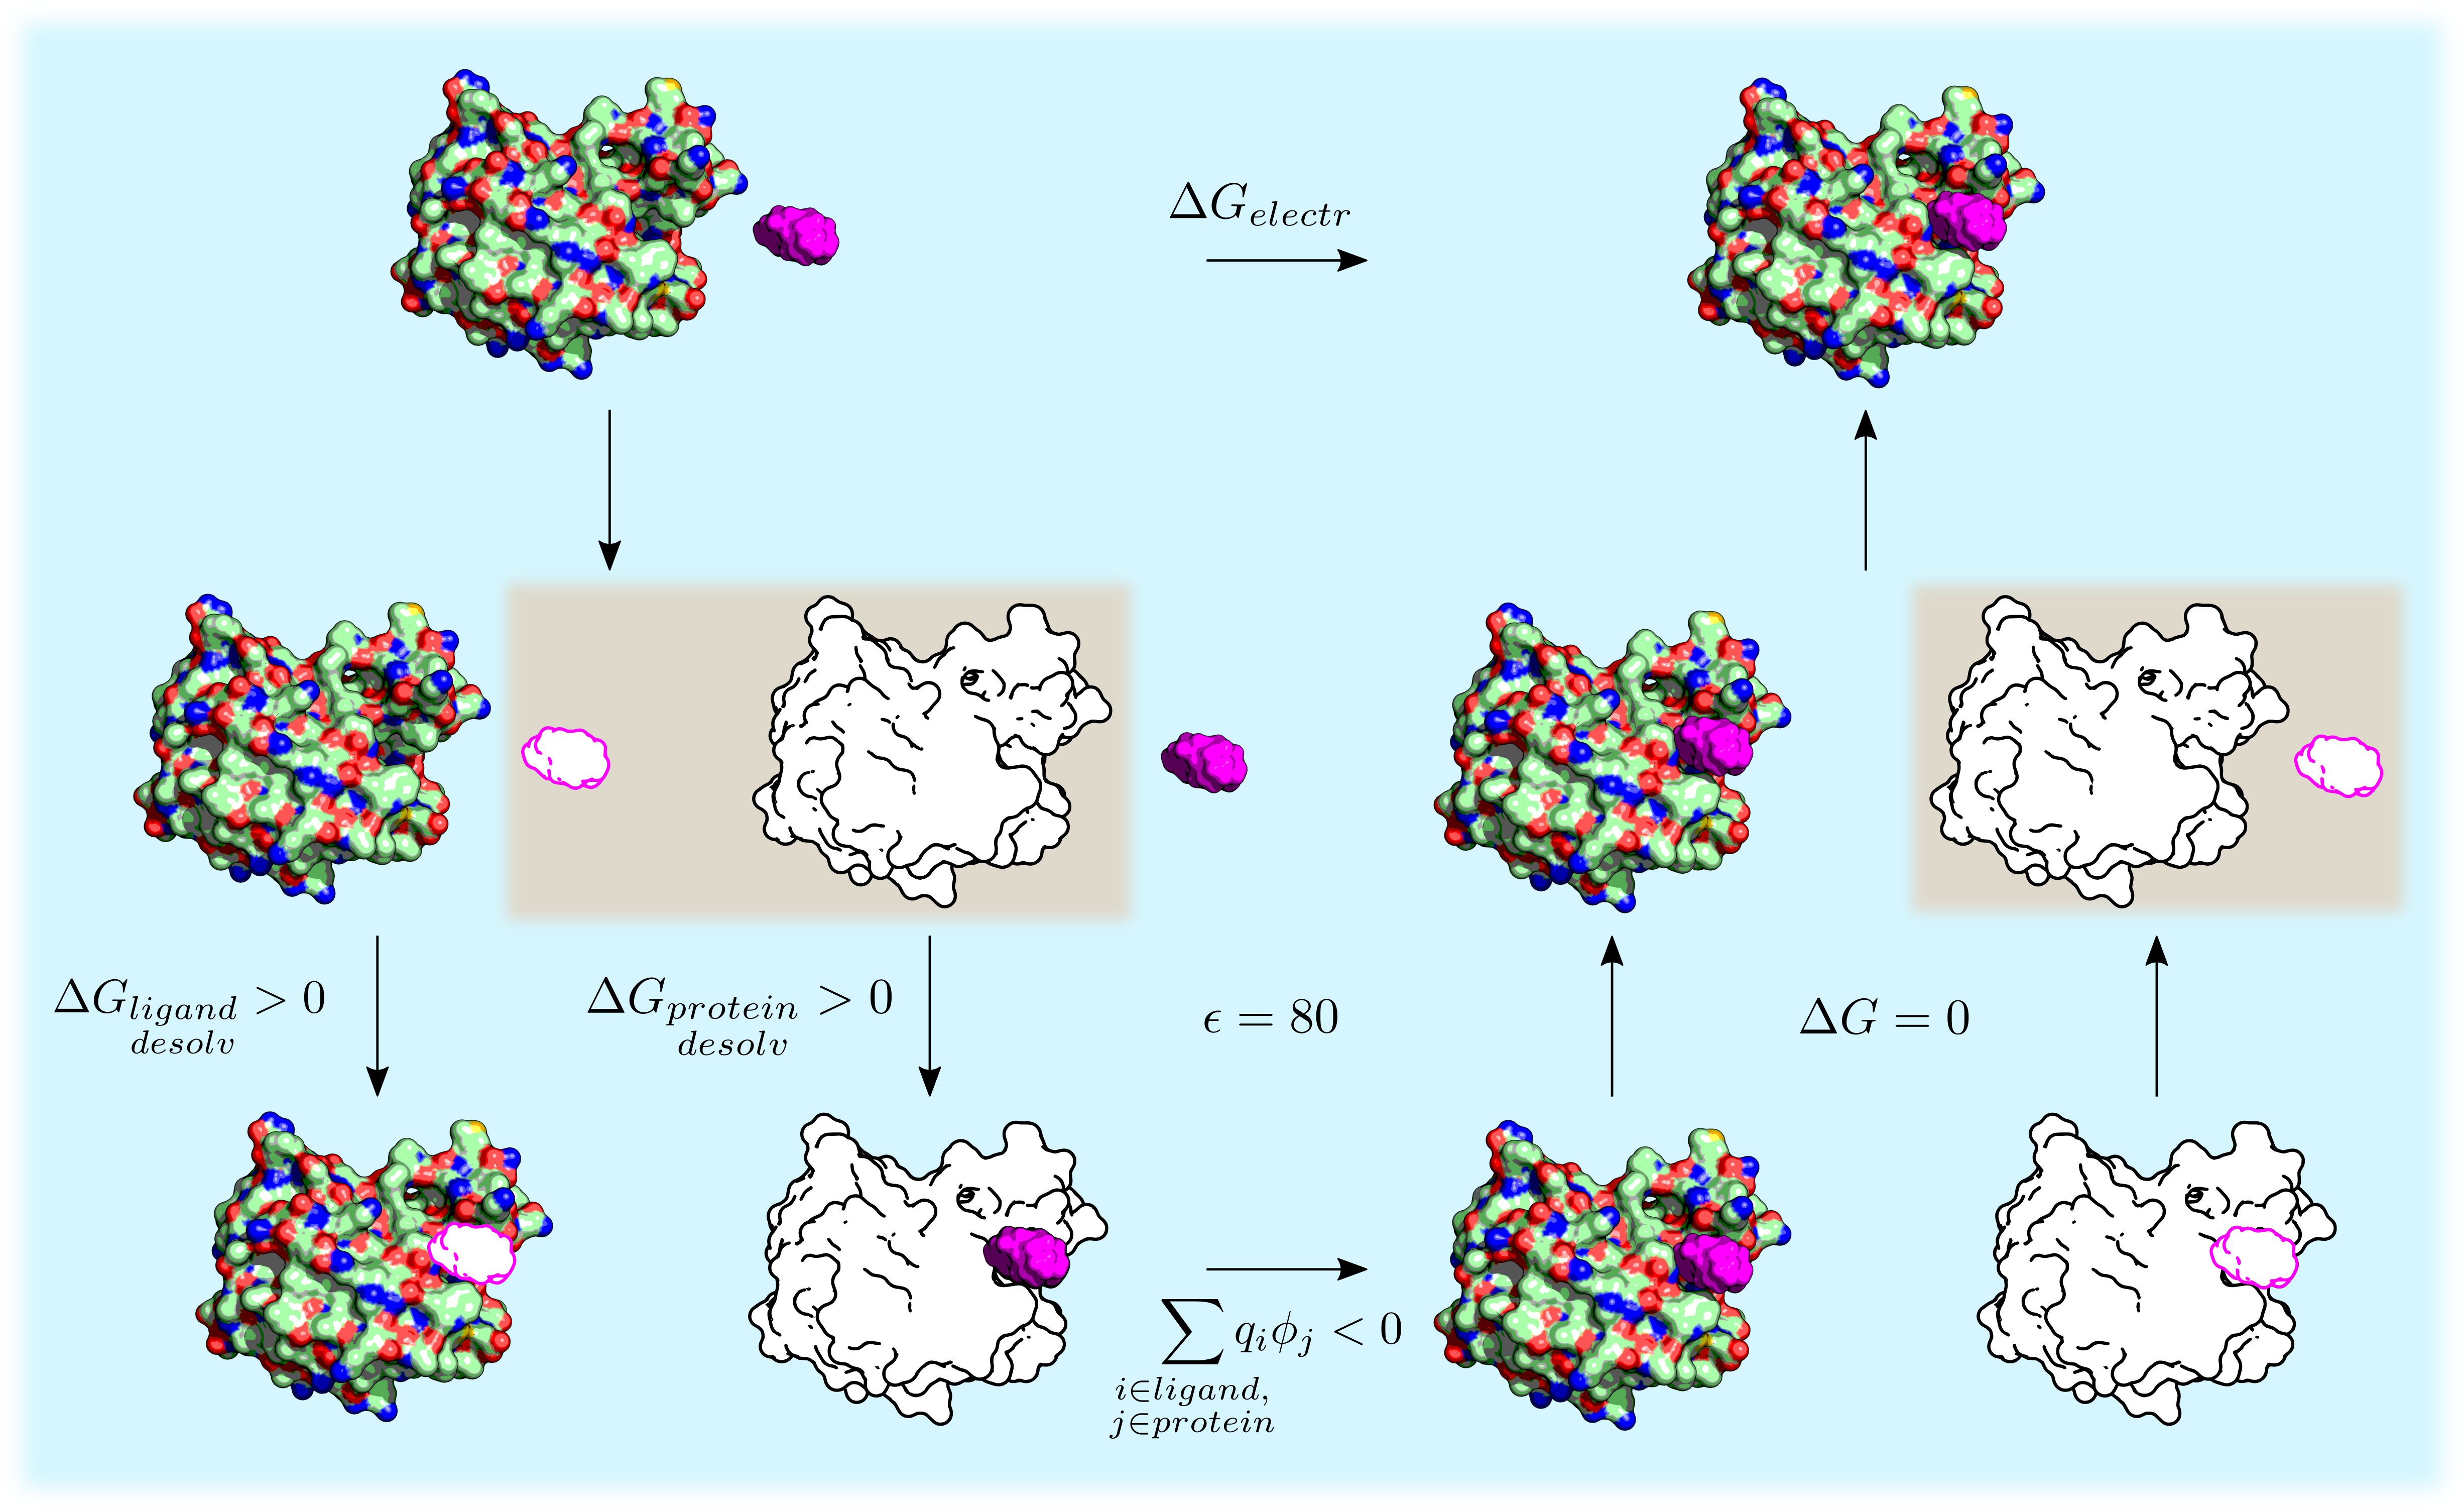
\includegraphics[scale=0.8]{figures/therm_cycle.png}
\makebox[\textwidth][c]{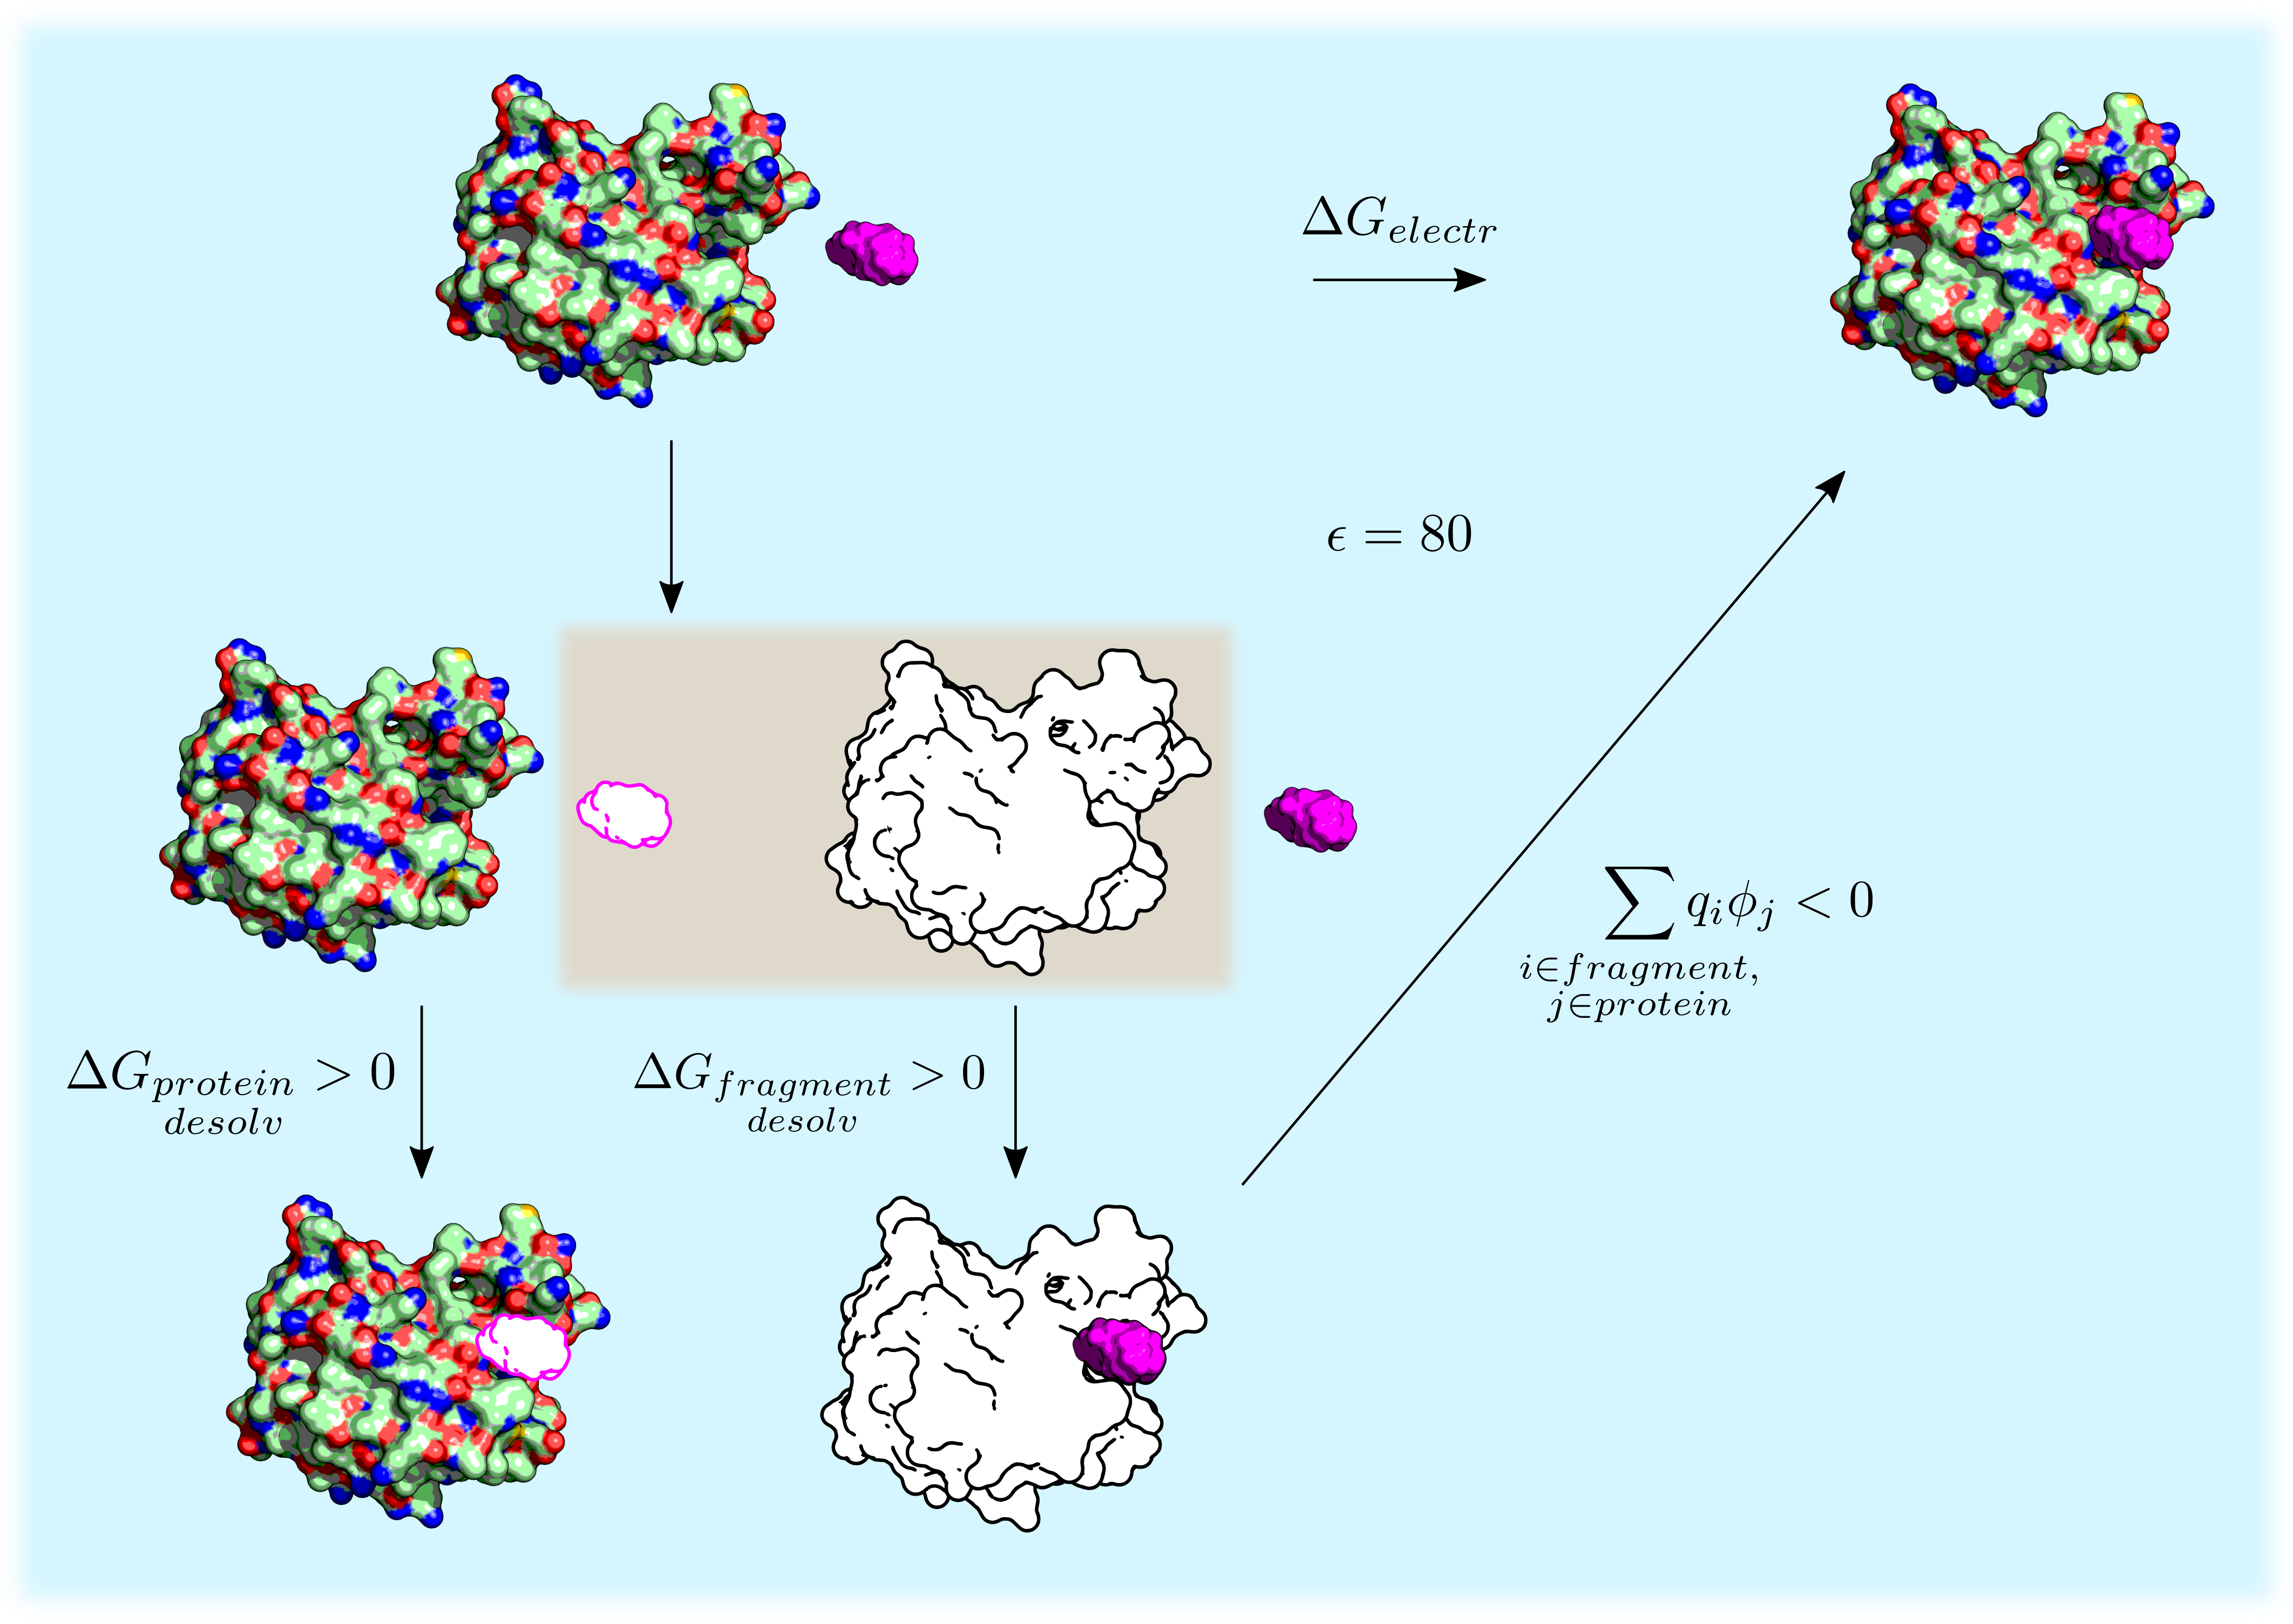
\includegraphics[width=1.1\textwidth]{figures/therm_cycle_reduced.png}}
%\end{center}
\caption{\textit{Decomposition of the electrostatic energy difference upon receptor-fragment binding $\Delta G_{electr}$. Charged solute is colored and uncharged solute is white. The fragment is in purple. The whole cycle takes place in water (blue background). The brown background box highlights the introduction of an uncharged copy of the solute.}}
\label{fig:thermo_cycle}
\end{figure}

\subsubsection{Accurate model}
\label{accurate:model}

\paragraph{Van der Waals interaction.}

A list of residue centroids is generated during the initial phase of the 
program and is used for an efficient estimation of van der Waals and screened 
electrostatic interactions.
The atom closest to the geometrical center of the residue
is selected as centroid for residues with zero
formal charge while the atom closest to the charge center is chosen for 
charged residues. The latter choice is more appropriate for the electrostatic 
interaction (see below). A 3D grid is built over the receptor with a distance 
between neighbor grid points of usually 1 \AA \, (set in the second term of {\bf p18}). 
Each centroid is assigned to the closest cubic element of the grid. Given a 
grid point $m$, all the grid points falling at a distance from $m$ smaller than 
a given cutoff (first term of {\bf p18}) define a pseudo-sphere associated to $m$.
The neighbor list of a given fragment atom contains the atoms belonging to the 
receptor 
residues whose centroid is included in the pseudo-sphere centered on the grid 
point closest to the fragment atom. This increases the efficiency because it 
avoids to calculate the distances between each fragment atom and all the 
receptor atoms when evaluating the interaction energy of a new fragment 
position. The van der Waals interaction energy is then 
computed between each atom of the fragment and the receptor atoms in the 
neighbor list according to 
\begin{eqnarray}
E^{\mbox{\tiny vdW}}_{ij} & = & \sqrt{\varepsilon_i \varepsilon_j} \left\{
                          \left( \frac{R^{\mbox{\tiny vdW}}_i + 
                          R^{\mbox{\tiny vdW}}_j}
                          {r_{ij}} \right)^{12} - 2 \left( 
                          \frac{R^{\mbox{\tiny vdW}}_i + 
                          R^{\mbox{\tiny vdW}}_j}{r_{ij}}
                          \right)^{6} \right\}
\end{eqnarray}
where $\varepsilon_i$ is the minimum of the van der Waals potential between 
two atoms of type $i$ at optimal distance of $2 \cdot R^{\mbox{\tiny vdW}}_i$. 
$R^{\mbox{\tiny vdW}}_i$ and $\varepsilon_i$ are specified in the 4th and 5th 
columns of {\bf p29}.

\paragraph{Partial desolvation of the receptor.}

The electrostatic energy in 
solution of the receptor can be expressed in terms of the 
electric displacement vector $\vec{D}\left(\vec{x}\right)$ and of a 
location dependent dielectric constant $\epsilon\left(\vec{x}\right)$ 
as an integral over three-dimensional space $R^3$:
%
\begin{equation}
%
E = {1\over {8\pi}} {\int_{R^{3}} {{\vec{D}^{2}\left(\vec{x}\right)}
\over {\epsilon\left(\vec{x}\right)}} \,d^{3}x}  
\label{eq:elen} 
%
\end{equation}
%
Since $\vec{D}\left(\vec{x}\right)$ is additive, for point charges it 
can be rewritten as a sum over all charges $i$ of the receptor: 
%
\begin{equation}
%
\vec{D}\left(\vec{x}\right) = 
\sum_{i} \vec{D}_{i}\left(\vec{x}\right) 
%
\end{equation}
%
Docking an uncharged molecular fragment in the receptor binding site 
has the only effect of modifying the 
dielectric properties of part of the binding site. Over the volume 
occupied by the fragment the dielectric constant changes from the 
solvent value ($\epsilon_{\mbox{\tiny w}}$) to the interior value 
($\epsilon_{\mbox{\tiny int}}$). 
The volume occupied by the fragment consists of the actual volume of the 
fragment and the interstitial volume enclosed by the reentrant surface between 
fragment and receptor (the first two terms of {\bf p18} are used for the 
construction of the SAS, i.e. solvent accessible surface, employed in this scheme). 
{\bf
In the limit in which the receptor electric displacement vector $\vec{D}$ 
does not change significantly upon fragment docking (i.e., for small fragments
and not close to a cluster of charges on the protein surface),} the variation of 
the electrostatic energy of the receptor can be written according to 
equation~\ref{eq:elen} as:
%
\begin{equation}
%
\Delta E = {\tau \over {8\pi} } {\int_{V_{frag}} 
{{\vec{D}^{2}\left(\vec{x}\right)}} \,d^{3}x}  
\label{eq:redeso} 
%
\end{equation}
%
where $\tau=\frac{1}{\epsilon_{\mbox{\tiny int}}} - \frac{1}{\epsilon_{\mbox{\tiny w}}}$ and $V_{frag}$ 
is the volume occupied by the fragment.
On a 3D grid equation~\ref{eq:redeso} becomes:
%
\begin{equation}
%
\Delta E = {\tau \over {8\pi} } {\sum_{k\in V_{frag}} 
{{\vec{D}^{2}\left(\vec{x_k}\right)}} \Delta V_k}  
\label{eq:redesogr} 
%
\end{equation}
%
The receptor electric displacement is calculated over a 3D grid 
(grid margin and spacing set in {\bf p20}) and it is approximated
by the Coulomb field 
%
\begin{equation}
%
\vec{D}\left(\vec{x}\right) = 
\sum_{i} q_i 
\ \frac{\left(\vec{x}-\vec{x_i}\right)} 
{\left|\vec{x}-\vec{x_i}\right| ^3} 
\label{eq:Dcoul} 
%
\end{equation}
%
This is an analytical approximation of the total electric 
displacement Alternatively, $\vec{D}$ can be calculated exactly for the isolated 
receptor by a finite difference solution of the Poisson equation and 
assumed not to change significantly upon fragment docking: 
%
\begin{equation}
%
\vec{D}\left(\vec{x}\right) = 
- \epsilon\left(\vec{x}\right) \nabla \phi\left(\vec{x}\right)
\label{eq:Dfd} 
%
\end{equation}
%
where $\phi$ is the electrostatic potential solution of the Poisson 
equation. This calculation is not available any longer within SEED.


\paragraph{Screened fragment-receptor interaction.}

The fragment-receptor interaction in solution is calculated 
via the GB approximation. 
The interaction energy in solution between two charges embedded in a solute is 
%
\begin{equation}
%
E^{int}_{ij} = \frac{q_i q_j}{\epsilon_{\mbox{\tiny int}} r_{ij}} - 
\frac{q_i q_j \tau}{R^{GB}_{ij}}
\label{eq:gb}
%
\end{equation}
%
where
%
\begin{equation}
%
 R^{GB}_{ij} = \sqrt{r_{ij}^{2} + R^{eff}_{i}R^{eff}_{j}
exp\left(\frac{-r_{ij}^{2}}{4R^{eff}_{i}R^{eff}_{j}}\right)}
\label{eq:rgb}
%
\end{equation}
%
$q_i$ is the value of the partial charge $i$, while
$r_{ij}$ is the distance between charge $i$ and $j$.
$R^{eff}_{i}$ is the effective radius of charge $i$ and it is 
evaluated numerically on a 3D grid covering the solute as described 
in~\cite{Scarsi:Continuum}.  It is a quantity depending only on the 
solute geometry and represents an estimate of the average distance of 
a charge from the solvent.

The intermolecular interaction energy is calculated as:
%
\begin{equation}
%
E^{int} = \sum_{{i \in fragment} \atop{j \in list_i}} E^{int}_{ij}
\label{eq:intwat}
%
\end{equation}
%
where ${list_i}$ contains the receptor atoms belonging to the neighbor 
list of fragment atom $i$. The electrostatic neighbor list includes all the receptor 
atoms of the van der Waals neighbor list (see above) 
and one atom for every charged residue whose 
centroid falls within a given cutoff (radius of the pseudo-sphere
increased by 30\%; {\bf p18}) 
of the binding site residues. The atom selected is the one closest to the 
center of charge. Supplementing the van der Waals neighbor list with a monopole 
approximation of distant charged residues dramatically reduces the error 
originating from the long range effects of electrostatics.

\paragraph{Partial desolvation of the fragment.}

The fragment intramolecular energy in solution is calculated with the 
GB formula as described in~\cite{Scarsi:Continuum}:
%
\begin{equation}
%
E = \sum_{i \in fragment} E^{self}_{i} 
+ \sum_{ {i > j} \atop{i,j \in fragment} } 
\left( \frac{q_i q_j}{\epsilon_{\mbox{\tiny int}} r_{ij}} - 
\frac{q_i q_j \tau}{R^{GB}_{ij}} \right)\\
\label{eq:enwat}
%
\end{equation}
%
where the two sums run over the partial charges of the fragment.
Equation~\ref{eq:enwat} differs from equation~\ref{eq:intwat} due to the 
presence of the {\it self-energy} term $\sum_{i} E^{self}_{i}$. This 
term is not zero only in the case of intramolecular energies. 
$E^{self}_{i}$ is the {\it self-energy} of charge $i$ and 
represents the interaction between the charge itself and the solvent. 
It is calculated as 
%
\begin{equation}
%
E^{self}_{i} = \frac{q^2_i}{2 R_{i}^{vdW} \epsilon_{\mbox{\tiny int}}}
- \frac{q^2_i \tau}{2 R^{eff}_{i}}
\label{eq:self}
%
\end{equation}
%
where $R_{i}^{vdW}$ is the van der Waals radius of charge $i$.

The difference in the intramolecular fragment energy upon binding 
to an uncharged receptor in solution is:
%
\begin{equation}
%
\Delta E = E^{docked} - E^{free}
\label{eq:frdeso}
%
\end{equation}
%
where $E^{docked}$ and $E^{free}$ are the energies of the fragment
bound and unbound to the receptor in solution, respectively. They are 
evaluated according to equation~\ref{eq:enwat}. For the unbound fragment 
($E^{free}$) the effective radii are calculated considering as solute the 
volume enclosed by the molecular surface of the fragment. 
For the bound fragment ($E^{docked}$) the solute is the volume enclosed by 
the molecular surface of the receptor-fragment complex. 
$E^{free}$ is evaluated only once per fragment type, while 
$E^{docked}$ is recalculated for every fragment position in the binding site.

\paragraph{Empirical correction term.}

(Modification of March 2003) $\;$
An empirical correction term (equation 8 in~\cite{Lee:Novel}) 
to the Coulomb field approximation in the generalized Born model is used for the accurate screened interaction and fragment desolvation 
energies. Protein desolvation does not use the GB model.

\subsubsection{Fast model}
\label{fast:model}

\paragraph{Van der Waals interaction.}

The van der Waals interaction between a fragment and the receptor is described 
as the sum of a steep repulsion and an attractive dispersion term with the 6-12
Lennard-Jones model:
\begin{equation}
E_{\mbox{\tiny vdW}} = \sum_{i \in \mbox{\tiny fragment}} 
                       \sum_{j \in \mbox{\tiny receptor}} 
                       \left( \frac{A_{ij}}{r^{12}_{ij}} - 
                              \frac{B_{ij}}{r^{6}_{ij}}
                       \right)
\label{eq:genvdW}
\end{equation}
where $r_{ij}$ is the distance between atoms $i$ and $j$, $A_{ij}$ and $B_{ij}$ 
are van der Waals repulsion and attraction parameters. The assumption that the 
receptor is rigid favors the use of a grid-based evaluation of the 
interaction. To make the fragment and receptor terms in equation 
(\ref{eq:genvdW}) factorizable, the geometric mean approximation is 
used: 
$A_{ij}=\sqrt{A_i A_j}$ and $B_{ij}=\sqrt{B_i B_j}$, 
with $A_{i}=\varepsilon_i(2R_i^{\mbox{\tiny vdW}})^{12}$ and 
$B_{i}=2\varepsilon_i(2R_i^{\mbox{\tiny vdW}})^6$. $R_i^{\mbox{\tiny vdW}}$ is 
the van der Waals radius of atom $i$ and $\varepsilon_i$ is the minimum of the 
van der Waals potential between two atoms of type $i$ at optimal distance of 
$2R^{\mbox{\tiny vdW}}_i$ ($R_i^{\mbox{\tiny vdW}}$ and $\varepsilon_i$ are specified 
in the 4th and 5th columns of {\bf p29}). 
A grid is spanned over the binding site of the 
receptor and the grid spacing is usually 0.2 \AA\ or 0.3 \AA \, (grid margin and spacing 
set in {\bf p17}). 
When the program starts, for every grid point $p$
the two following "receptor potentials" are calculated and stored in
look-up tables: 
\begin{eqnarray}
\phi^A(p) = \sum_{j \in \mbox{\tiny receptor}} \frac{\sqrt{A_j}}{r_{pj}^{12}} 
& \,\,\,\,\,\, \mbox{and} \,\,\,\,\,\,  &
\phi^B(p) = \sum_{j \in \mbox{\tiny receptor}} \frac{\sqrt{B_j}}{r_{pj}^6} 
\label{eq:twoval}
\end{eqnarray}
where the sums run over the receptor atoms which are within a 10 \AA $\:$ 
cutoff distance of the grid point. The contribution of fragment atom $i$ with
coordinates
$\vec{x}_i$ is evaluated by multiplying its van der Waals parameters 
($\sqrt{A_i}$ and $\sqrt{B_i}$) with the 
"receptor potentials"  ($\phi^A$ and $\phi^B$, respectively).
The value of the potential is
derived from the eight points of the grid surrounding $\vec{x}_i$ by the 
trilinear interpolation method~\cite{Press:Numerical}.

\paragraph{Partial desolvation of the receptor.}

A preliminary step consists of the evaluation of the receptor desolvation 
due to a low dielectric probe sphere of 1.4 \AA\ radius rolling over the
van der Waals surface of the receptor. 
The center of the sphere spans the solvent accessible surface 
(SAS). A number of points are distributed uniformly on 
the SAS of the receptor with a given surface density (usually 0.5 points 
per \AA$^2$, see below) 
to describe the different positions of the center of the 
probe sphere.  Furthermore, a cubic grid of 0.5 \AA~spacing 
is used to discretize the volume surrounding the receptor.  The volume
occupied by the probe sphere is then approximated on the cubic grid.
\begin{figure}
\begin{center}
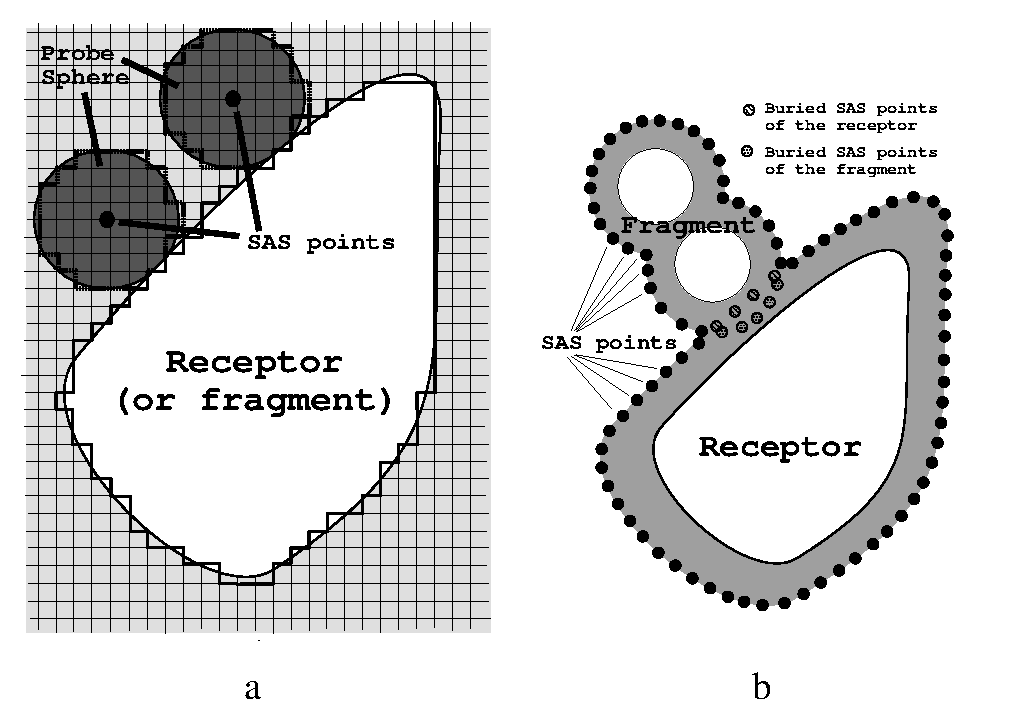
\includegraphics[scale=0.9]{figures/fig2.ps}
\end{center}
\caption{\it
(a) Evaluation of the receptor (fragment) desolvation due to a probe sphere 
rolling over the van der Waals surface of the receptor (fragment). A grid box of
0.5 \AA~spacing (light 
gray) is built around the molecule and the desolvation resulting from the 
occupation of every grid element is evaluated as described 
in~\cite{Majeux:Exhaustive}. The desolvation due to the probe sphere in a 
given position is approximated by the sum of the values of the desolvation due to
the cubes within the sphere (dark gray).
(b) Evaluation of the receptor and fragment desolvations upon binding. The 
points on the SAS of the receptor and the SAS of the fragment represent the 
positions of the rolling probe sphere. The receptor desolvation is approximated 
by the sum of the desolvation values associated with the SAS points of the 
receptor buried within the SAS of the fragment. The fragment desolvation is 
approximated by the sum of the desolvation values associated with the SAS 
points of the fragment buried within the SAS of the receptor.
}
\end{figure}
The receptor desolvation resulting from the probe sphere
at a point $p$ on the SAS of the receptor
(see Figure~5a) is evaluated according to the Coulomb approximation of the 
electric displacement: 
%
\begin{equation}
%
\Delta G^{p}_{\mbox{\tiny desolv}} = {1 \over {8\pi} } 
(\frac{1}{\epsilon_{\mbox{\tiny int}}} - \frac{1}{\epsilon_{\mbox {\tiny w}}}) 
{\sum_{k_p \in V_{probe}} \left( \sum_{j \in {\small receptor}} q_j 
\ \frac{\left(\vec{x}_{k_p}-\vec{x_j}\right)} 
{\left|\vec{x}_{k_p}-\vec{x_j}\right| ^3} \right)^2  \Delta V}  
\label{eq:redesofinal} 
%
\end{equation}
%
where the index $k_p$ runs over the cubic grid elements occupied by the probe
sphere and $\Delta V$ is the volume of a cube.  
Further, $\vec{x_j}$ is the coordinate vector of the receptor atom $j$,
$\vec{x}_{k_p}$ the position of the cube included in the probe sphere,
and $\epsilon_{\mbox{\tiny int}}$ and ${\epsilon_{\mbox {\tiny w}}}$ 
are the solute and
solvent dielectric constants, respectively.
The receptor desolvation due to the probe sphere is calculated only once 
at the beginning of SEED for every point on the SAS.  It is always
positive, i.e., unfavorable, because $\epsilon_{\mbox{\tiny int}} 
< {\epsilon_{\mbox {\tiny w}}}$.

The receptor desolvation upon binding
is approximated by the sum of the values of the desolvation operated by the 
probe sphere over the SAS receptor points that are included within the 
SAS of the fragment (see Figure~3b): 
%
\begin{equation}
%
\Delta G^{\mbox{\tiny receptor}}_{\mbox{\tiny desolv}} =
{\sum_{ p \in {\mbox{\small SAS}_{\tiny receptor}^{\tiny buried}} }
 \Delta G^{p}_{\mbox{\tiny desolv}}}
%
\end{equation}
%
Since the adjacent positions of the 
sphere can partially overlap, the total receptor desolvation is scaled by a 
multiplicative factor~\cite{Majeux:Efficient}. 
The assumption underlying this model is that the main contribution to the 
receptor desolvation results from the removal of the first shell of water. 
This approximation is justified by the fact 
that the desolvation of a spherical ion by a small low dielectric sphere at a 
distance $r$ from the ion varies as $\frac{1}{r^4}$.

\paragraph{Screened fragment-receptor interaction.}

The screened interaction between fragment and receptor 
($E^{\mbox{\tiny interm}}_{\mbox{\tiny elect}}$ in kcal/mol)
is calculated according to a linear 
distance-dependent dielectric model (first term of {\bf p16}):
%
\begin{equation}
%
E^{\mbox{\tiny interm}}_{\mbox{\tiny elect}} \, = \, \, \, 
332 \sum_{{i \in fragment} \atop{j \in receptor}} 
\frac{q_i q_j}{\epsilon_{\mbox{\tiny int}} r_{ij}^2} 
\label{eq:int}
%
\end{equation}
%
where $q_i$ and $q_j$ are the partial charges (in electronic units) 
of atoms $i$ and $j$, $r_{ij}$ is 
the distance between them (in \AA), 
and $\epsilon_{\mbox{\tiny int}}$ 
is the value of the interior, i.e., solute, dielectric constant ({\bf p1}). 
The calculation is done on a grid with trilinear interpolation. 
The grid margin and spacing are specified in {\bf p16}.

\paragraph{Partial desolvation of the fragment.}

The desolvation of the fragment 
($\Delta G^{\mbox{\tiny fragment}}_{\mbox{\tiny desolv}}$) 
is evaluated in a way that is specular to the 
receptor desolvation (see Figures~3a~and~3b). First, the fragment desolvation 
due to a probe sphere rolling over the fragment SAS is calculated once for 
every fragment type. Subsequently, the fragment desolvation upon binding is 
approximated by the sum of the desolvation values associated with the points 
on the SAS of the fragment that are included within the SAS of the receptor. 
The same scaling factor as for the receptor desolvation is employed~\cite{Majeux:Efficient}. 


\subsection{Docking scheme}
\label{ssec:Docking}

% OLDER VERSION OF DOCUMENTATION
% There are three docking schemes that the user can select in {\bf p13}: a relatively slow scheme using 
% the accurate energy, a faster scheme using the fast energy model and a two-step 
% procedure called postprocess scheme. 
% It is most convenient and appropriate to use the postprocess scheme in most projects. 
% If the hardware resources allow for it, one can use directly the accurate 
% docking scheme (i.e., skip the evaluation of the fast energy). 
% The fast docking scheme alone should not be used 
% because its energy evaluation is very approximative.

% NEWER VERSION
In order to efficiently speed up the screening of fragments, SEED relies on a two-step docking 
workflow we will refer to as postprocess scheme (see Figure 6); each part of it is detailed
below in the corresponding subsections.

\par In the first step, after the initial alignment of the fragment to a reference frame (pre-alignment of the fragment \ref{sssec:prealign}), 
the generated poses are screened and filtered according to the fast energy model 
(fast docking scheme \ref{sssec:fastdock}). Poses passing all the filters are 
sorted according to their
binding energy and clustered in order to find the most representative ones and discard redundant 
positions (clustering procedure \ref{sssec:Clustering}). 
\par In the second step the best binding modes within each cluster 
are rescored and ranked with the more accurate solvation model (accurate rescoring \ref{sssec:accurescore}).

%This protocol consists in the fast energy evaluation of the poses (fast docking scheme \ref{sssec:fastdock}); the generated positions are then clustered and sorted according to their binding energy and the best scoring poses are finally ranked according to the slow energy evaluation (accurate docking scheme \ref{sssec:accurdock}). 

\subsubsection{Pre-alignment of the fragment} %Added by Cassiano Langini
\label{sssec:prealign}
Before starting the docking procedure the fragment 
%can be optionally (parameter \textbf{pXXX})
is pre-aligned to a reference frame. The first atom of the fragment is put in the origin, the second is put along the positive \textit{x} axis, the third in the \textit{xy} plane and the others are aligned accordingly. If the third atom is collinear with the first two, the fourth atom is considered and so on. As the positioning of points on the Solvent Accessible Surface has a dependency on the absolute orientation of the fragment, the pre-alignment step is necessary to ensure consistency of results when docking (first line of \textbf{i7} set to \texttt{d}) the same fragment provided in different spatial orientations or when carrying out an energy evaluation (first line of \textbf{i7} set to \texttt{e}) of a fragment previously docked by SEED. Residual differences may be due to the limited precision of coordinates in usual mol2 files.
%Differences in results without the pre-alignment should become less relevant if the density of apolar vectors (\textbf{pXXX}) is increased. 
% When carrying out energy evaluation without docking (\textbf{pXXX} set to \texttt{y}) on a pose generated by seed, pre-alignment should be used in both the posing and the energy evaluation calculation.

%\subsubsection{Postprocess scheme}
%\label{sssec:Post}
%An efficient way of speeding up the fragment screening by SEED is to divide the selection of favorable 
%binding modes into two separate steps (see Figure 4). In the first step, the fast docking scheme
%is used (see \ref{sssec:fastdock} below). The positions are then sorted according to binding energy 
%and clustered (see below {\bf Clustering procedure}). 
%In the second step, the $n$ best binding modes ($n$ is set in {\bf p5}) within each cluster are 
%evaluated with the more accurate solvation model (see \ref{accurate:model}).

\subsubsection{Fast docking scheme}
\label{sssec:fastdock}

The fast docking scheme proceeds by applying sequentially the following filters:

\begin{enumerate}

\item {\it Sphere for acceptance of the fragment position.}
This filter is optional. The user can specify a sphere (coordinates of the center and radius in 
{\bf i6}) in which the geometry center of the fragment position must be to be accepted.

\item {\it Van der Waals interaction used as bad contacts detection.}
The fast van der Waals energy is used to detect clashes: 
a fragment is discarded if it is less favorable than a threshold value set in {\bf p11}.

\item {\it Van der Waals interaction for apolar docking.}
To increase efficiency apolar fragments are discarded without evaluation of the electrostatic 
contribution if the fast van der Waals interaction is less favorable than a threshold value. This value is 
calculated by multiplying {\bf p19} by the number of fragment atoms.

\item {\it Total energy.}
The fragment position is finally accepted if the total energy (fast model) is smaller than a cutoff 
given in the 
third column of {\bf i7}. The total energy is the sum of the van der Waals interaction energy plus 
the electrostatic contribution (screened intermolecular energy and protein and fragment desolvation 
terms). These four terms can be weighted by the scaling factors in {\bf p23}.

\end{enumerate}

\begin{comment}
% This scheme is no longer availble!!!
\subsubsection{Accurate docking scheme}
\label{sssec:accurdock}

The accurate docking scheme proceeds by applying sequentially the following filters:

\begin{enumerate}

\item {\it Sphere for acceptance of the fragment position.}
This filter is optional. The user can specify a sphere (coordinates of the center and radius in 
{\bf i6}) in which the geometry center of the fragment position must be to be accepted.

\item {\it Bad contacts detection.}
A grid is defined over the whole receptor. This is followed by the generation of a list which contains 
for every cubic grid element the atoms which are enclosed by the surface of the cubic element. This list 
is calculated only once at the beginning of the program and is used to check bad contacts. A bad 
contact is defined as $r_{ij} < \alpha (R_i^{\mbox{\tiny vdW}}+R_j^{\mbox{\tiny vdW}})$ and a severe 
overlap is defined as $r_{ij} < \alpha \beta (R_i^{\mbox{\tiny vdW}}+R_j^{\mbox{\tiny vdW}})$, where 
$r_{ij}$ is the distance between two atoms ($i \in$ fragment, $j \in$ receptor), and 
$R_i^{\mbox{\tiny vdW}}$ and $R_j^{\mbox{\tiny vdW}}$ are the corresponding van der Waals radii. The 
value of $\alpha$ is usually set to $2^{-1/6}=0.89$ (second term of {\bf p10}), the distance at which 
repulsion balances attraction, and a $\beta$ of 0.6 (third term of {\bf p10}) is employed normally. 
The distances between an atom of the fragment and the receptor atoms in the 27 grid cubes 
surrounding the fragment atom are calculated. This is repeated for every atom in the fragment. A grid spacing of 
twice the largest van der Waals radius is used to avoid missing clashes. For polar fragments the 
hydrogen atom involved in the H-bond is not checked for bad contacts. Fragments with one severe overlap 
or a number of bad contacts larger than a cutoff are discarded. This cutoff is the number of 
fragment atoms multiplied by the number given in the first term of {\bf p10}.

\item {\it Van der Waals interaction for apolar docking.}
To increase efficiency apolar fragments are discarded without evaluation of the electrostatic 
contribution if the van der Waals interaction (accurate model) is less favorable than a threshold 
value. This value is 
calculated by multiplying {\bf p19} by the number of fragment atoms.

\item {\it Total energy.}
The fragment position is finally accepted if the total energy (accurate model) is smaller than a cutoff 
given in the 
third column of {\bf i7}. The total energy is the sum of the van der Waals interaction energy plus 
the electrostatic contribution (screened intermolecular energy and protein and fragment desolvation 
terms). These four terms can be weighted by the scaling factors in {\bf p23}.

\end{enumerate}
\end{comment}

\subsubsection{Clustering procedure}
\label{sssec:Clustering}

The docking of a given fragment (with energy evaluation as 
described above) is followed by sorting and clustering.  Within each fragment type, 
positions are first sorted according to binding energy.  Positions
whose binding energy is lower than a user-specified threshold value 
(see filter 4. in \ref{sssec:fastdock}) are
then clustered (a maximal number of positions can be set in {\bf p27}) using as similarity criterion 
between two fragment positions $A$ and $B$: 
\begin{eqnarray}
S(A,B)=\frac{S_{AB}}{\max (S_{AA},S_{BB})} & \mbox{ where } & 
    S_{XY}=\sum_{i \in X} \sum_{j \in Y} w_{t_i t_j} \exp (- \gamma r^2_{ij})
\end{eqnarray}
where
$r_{ij}$ is the distance between two atoms ($i \in$ fragment position $X$, 
$j \in Y$), $w_{t_i t_j}$ is a user-controlled matrix whose coefficients 
reflect the similarity between element types (in most cases a unit matrix is used; 
otherwise the non-default coefficients have to be set in {\bf p24} by giving the number of non-default 
values on the first line and two element types with the non-default value on the following lines) 
and $\gamma$ is a coefficient which acts on the broadness of the distribution
of the positions.  $B$ is assigned to the cluster of 
$A$ if $S(A,B)$ is larger than a cutoff value $\delta$ with $0 \leq \delta \leq 
1$. 
The clustering proceeds in two steps :
(1) a first clustering with $\gamma=0.9$ (first term of {\bf p25}) and $\delta=0.4$ 
(second term of {\bf p25}) yields 
large clusters which contain almost overlapping as well as more distant fragments; 
(2) a second clustering with $\gamma=0.9$ (first term of {\bf p26}) and $\delta=0.9$ 
(second term of {\bf p26}) is done on each 
cluster found in (1) to eliminate fragments which are very close in space. 
The second clustering is applied on the positions for which the binding energy of the representative 
is smaller than a cutoff value specified in the 4th column of {\bf i7}. 
A single clustering step with $\gamma=0.9$ and $\delta=0.9$ would generate 
too many small clusters. Hence, the first step is a real clustering while the 
second step is done only to discard redundant positions. 

\subsubsection{Accurate rescoring}
\label{sssec:accurescore}
The $n$ best binding modes within each cluster ($n$ is set in {\bf p5}) are rescored and ranked 
according to the accurate solvation model. Note that it is possible that poses passing the total
energy filter during fast docking result in a binding energy above the cutoff (set in the 3rd column of {\bf i7}) with the accurate model. These poses 
appears in the docking summary in the {\tt seed.out} log, but are not written to any other
output files of the postprocess scheme (see \ref{sssec:PostproOut}).

\begin{figure}
\vspace*{-1in}
\begin{center}
\makebox[\textwidth][c]{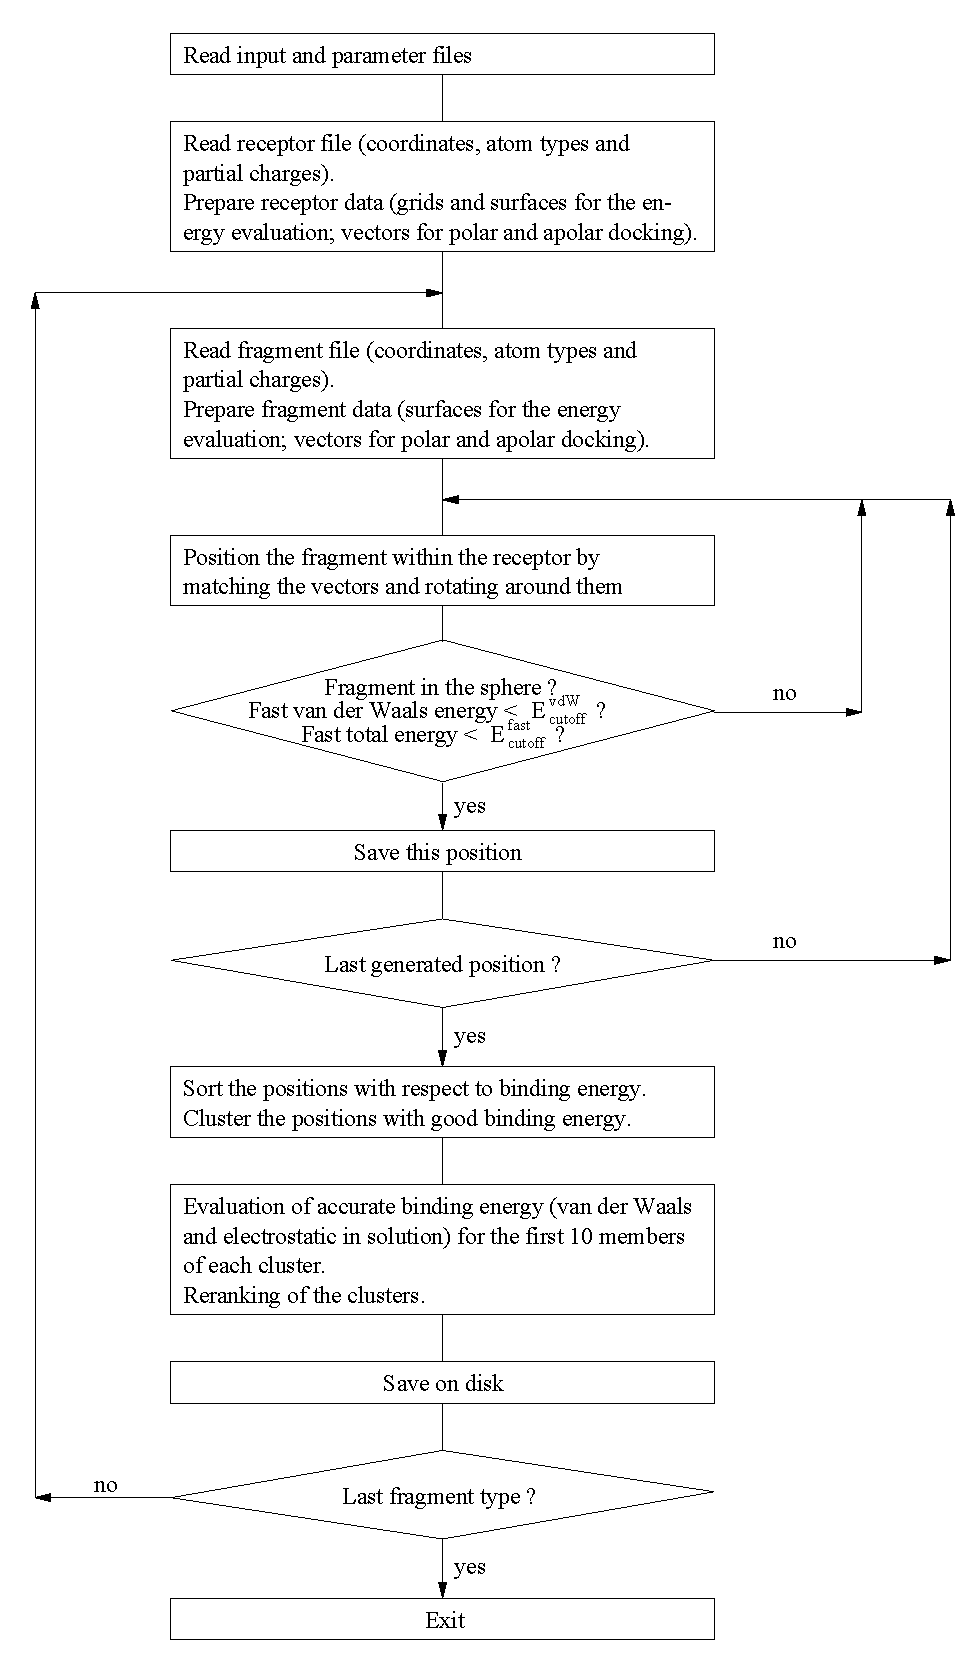
\includegraphics[scale=0.8]{figures/fig3_final.pdf}}
\end{center}
\caption{\it Schematic representation of the SEED program (postprocess scheme).}
\end{figure} 

%\subsection{Geometrical centers for FFLD}
%\label{ssec:Geometrical}

%The geometrical centers that are used in FFLD~\cite{Budin:Fragment} to guide 
%the docking of flexible fragments are built as follows~\cite{Cecchini:Automated}. 
%Cluster representatives resulting from the postprocess scheme are 
%subsequently grouped according to the
%coordinates of their geometrical centers using a threshold of 
%{\bf p28} (fourth term) \AA.
%The geometrical centers of the first {\bf p28} (third term) cluster 
%representatives are removed and directly used for docking. The remaining 
%geometrical centers are again grouped according to the same threshold. 
%For each cluster an average geometrical 
%center ($\mathbf r_{AGC}$) is calculated with the following
%procedure. First, all the positions with a binding energy greater than
%{\bf p28} (fifth term) kcal/mol with respect to the cluster representative 
%are discarded.
%Then, the $\mathbf r_{AGC}$ of a given cluster is evaluated as an
%energy weighted mean

%\vspace{-1cm}
%\begin{equation}
%{\mathbf r_{AGC}} = \sum_{i=1}^{N} \omega_{i} {\mathbf r_{i}}\, \quad
%\label{eq:geomcent1}
%\end{equation}

%\vspace{-0.5cm}
%\begin{equation}
%\omega_{i} = \left\{
%\begin{array}{ll}
%E_{i}\; / \;\sum_{i} E_{i} & \quad \textrm{if} \quad E_{max} < 0 \\
%(E_{i} - (E_{min} + E_{max})\;) \; / \;\sum_{i} (E_{i} - (E_{min} + 
%E_{max})\;) & \quad \textrm{if} \quad E_{min} > 0
%\end{array} \right.
%\end{equation}
%\noindent
%where $E_{min}$ and $E_{max}$ are the minimum and maximum energy
%within a cluster, respectively, and the sum runs over the $N$
%geometrical centers $\mathbf r_{i}$ of the fragments in the
%cluster. In the sporadic case of $E_{min} > 0$, by subtracting
%$(E_{min} + E_{max})$ from the fragment binding energies $E_{i}$, it
%is possible to give more weight to positions with small absolute
%energy values. For $E_{min} \le 0 \le E_{max}$, average centers for
%the subsets of favorable ($E_{i} < 0$) and unfavorable ($E_{i} > 0$)
%binding modes in a cluster ($\mathbf r_{-}$ and $\mathbf r_{+}$,
%respectively) are computed by equation~\ref{eq:geomcent1} 
%and the $\mathbf r_{AGC}$ is evaluated as

%\vspace{-1cm}
%\begin{equation}
%{\mathbf r_{AGC}} = {\alpha_{-} \; \mathbf r_{-}} + \alpha_{+} \; 
%{\mathbf r_{+}}
%\end{equation}
%\noindent
%where $\alpha_{-}$ and $\alpha_{+}$ (sixth and seventh terms of 
%{\bf p28}, respectively) are multiplicative factors. 
%The final list of geometrical centers used for docking is a compromise 
%between the accuracy of the SEED binding energy 
%(geometrical centers of {\bf p28} (third term) cluster representatives 
%optimally docked by SEED) and the diversity derived from the clustering 
%procedure (average geometrical centers).
%The post-processing of the optimal binding modes of the
%fragments leads to more heterogeneous binding site maps than using
%only the most favorable ones. 

%\noindent
%This post-processing is activated or deactivated by the first 
%term of {\bf p28}.

\subsection{Energy evaluation mode}
\label{ssec:Energy}

SEED allows the energy of a particular fragment position to be evaluated without using the docking mode. 
{\bf i7} has to be set to {\tt e} (energy evaluation mode) instead of {\tt d} (docking mode). 
The fragment mol2 file must contain the coordinates of the relevant position, for which the binding energy has to be evaluated.

\subsection{SEED output files}

The grids for fast van der Waals energy, fast screened interaction energy and receptor desolvation 
can be saved on disk and reused for a subsequent run ({\bf p7},{\bf p8},{\bf p9}). 
The path of the main output file of SEED is set in {\bf i6}. The first term of {\bf p28} is the 
maximal number of lines that can be written in the main output file for each docking step of each 
fragment type. The second term of {\bf p28} gives control on which information may be discarded 
in the output file.

\noindent
A directory {\tt outputs} in which most of the output files are written is automatically 
created by the program.

\noindent
{\tt apolar\_rec.mol2} and {\tt apolar\_rec\_reduc.mol2} contain the apolar vectors before and 
after reduction ({\bf p2}), respectively. 
{\tt apolar\_rec\_reduc\_angle.mol2} contains the vectors of {\tt apolar\_rec.mol2} which are 
selected if the angle criterion ({\bf i4}, {\bf p14}) is activated.
The polar vectors are in {\tt polar\_rec.mol2}, {\tt polar\_rec\_reduc\_angle.mol2}, and 
{\tt polar\_rec\_reduc.mol2}.

\noindent
Out of the vectors that passed the angle reduction criterion, \textbf{p2} selects the percentage of them that should be used for docking (first value for polar and second for apolar vectors). The CPU time required by SEED is proportional to these numbers.
%Maximal number of selected polar and apolar vectors, respectively. The CPU time 
%required by SEED is proportional to these numbers.


\subsubsection{Postprocess scheme}
\label{sssec:PostproOut}

{\tt $<$FragmentMol2FileName$>$\_clus.mol2} contains the top poses per cluster 
ranked by accurate energy.  It is a mol2 file and includes the hydrogen atoms. See \ref{ssec:MostOut} for details.
%In the {\tt @$<$TRIPOS$>$SUBSTRUCTURE} section the 
%cluster numbering and total accurate energies are stored in the third and second last 
%columns (for the computer programs FFLD~\cite{Budin:Fragment} and SLD, unpublished).

\noindent
{\tt $<$FragmentMol2FileName$>$\_best.mol2} contains the top poses 
ranked by accurate energy. See \ref{ssec:MostOut} for details.

\noindent
\texttt{seed\_clus.dat} is a summary table containing all the relevant energy terms corresponding to the poses saved in {\tt $<$FragmentMol2FileName$>$\_clus.mol2}. See \ref{ssec:MostOut} for details.

\noindent
\texttt{seed\_best.dat} is a summary table containing all the relevant energy terms corresponding to the poses saved in {\tt $<$FragmentMol2FileName$>$\_best.mol2}. See \ref{ssec:MostOut} for details.

%\noindent
%{\tt FragmentName\_clus\_pprocr.chm} 
%contains the representatives of the clusters, 
%i.e., the top pose (ranked by accurate energy) within each cluster.
%(It is a CHARMM-format file 
%for visualization with the molecular modeling program WITNOTP; A. Widmer, unpublished).

%\noindent
%{\tt FragmentName\_clus\_pproc.chm} is the same as {\tt FragmentName\_clus\_pproc.mol2} 
%but in CHARMM format. (Only the coordinates of the heavy atoms are included 
%for CCLD~\cite{Caflisch:ccld}).

%\noindent
%{\tt FragmentName\_geomcent.mol2} contains the geometrical centers for 
%FFLD (see \ref{ssec:Geometrical}). 
%The right-hand column contains their corresponding energies. 
%The first {\bf p28} (third term) geometrical centers are characterized 
%by zinc atoms, the remaining geometrical centers by chlorine atoms. 
%The second term of {\bf p28} is the maximal number of geometrical centers 
%to write in this file.

\par
The writing of the above {\tt *\_clus.mol2}  and \texttt{*\_best.mol2} file is activated or deactivated 
by {\bf p3} (first and second value respectively). The writing of the \texttt{*\_clus.dat} and \texttt{*\_best.dat} summary table is activated or deactivated by \textbf{p4} (first and second value respectively). 
The maximum number of positions saved is specified in \textbf{p5}; 
the first value corresponds to the number of cluster members 
(\textit{i. e.} number of poses per cluster) 
and the second to the total number of best poses, independently of the cluster they come from 
(see \ref{ssec:MostOut} for details). Note that these are upper bounds as the number of 
generated poses may be smaller
than the number of poses requested in output. 
All the four parameters for writing the output files (\textbf{p3} and \textbf{p4}) can be switched on/off independently.

%\subsubsection{Accurate docking scheme}
%\label{accuratedocking:scheme}

%\noindent
%{\tt FragmentName.chm} contains the top 999 poses ranked by accurate energy. 

%\noindent
%{\tt FragmentName\_clus.chm} contains the top 999 positions before clustering.
%Only the coordinates of the heavy atoms are included (for the computer program CCLD).

%\noindent
%{\tt FragmentName\_clus\_reduc.chm} contains the fragment positions of the top clusters up to 
%999 positions with a limited number ({\bf i4}) of positions per cluster. Only the coordinates %of 
%the heavy atoms are included (for CCLD).

%\noindent
%{\tt FragmentName\_xxx.mol2} are xxx files, each with a single pose where xxx=1 is the top pose
%according to accurate energy, xxx=2 is the second best pose, etc.
%The total number of this type of file is limited to {\bf p12} (which is usually set to 1).

%\subsubsection{Fast docking scheme}

%It is used in the postprocessing scheme.  Note that the fast docking scheme
%should not be run alone except for debugging purposes.
%{\tt FragmentName.chm}, {\tt FragmentName\_clus.chm}, {\tt FragmentName\_clus\_reduc.chm} and 
%{\tt FragmentName\_xxx.mol2} are the same as for the accurate docking scheme 
%(see \ref{accuratedocking:scheme}) but with the fast energy.

\newpage

\bibliography{a-bib}

%\newpage

\section*{}
\addcontentsline{toc}{figure}{Parameter file}


\begin{figure}[p]
\vspace*{-1.2in}
  \centering
  \makebox[\textwidth][c]{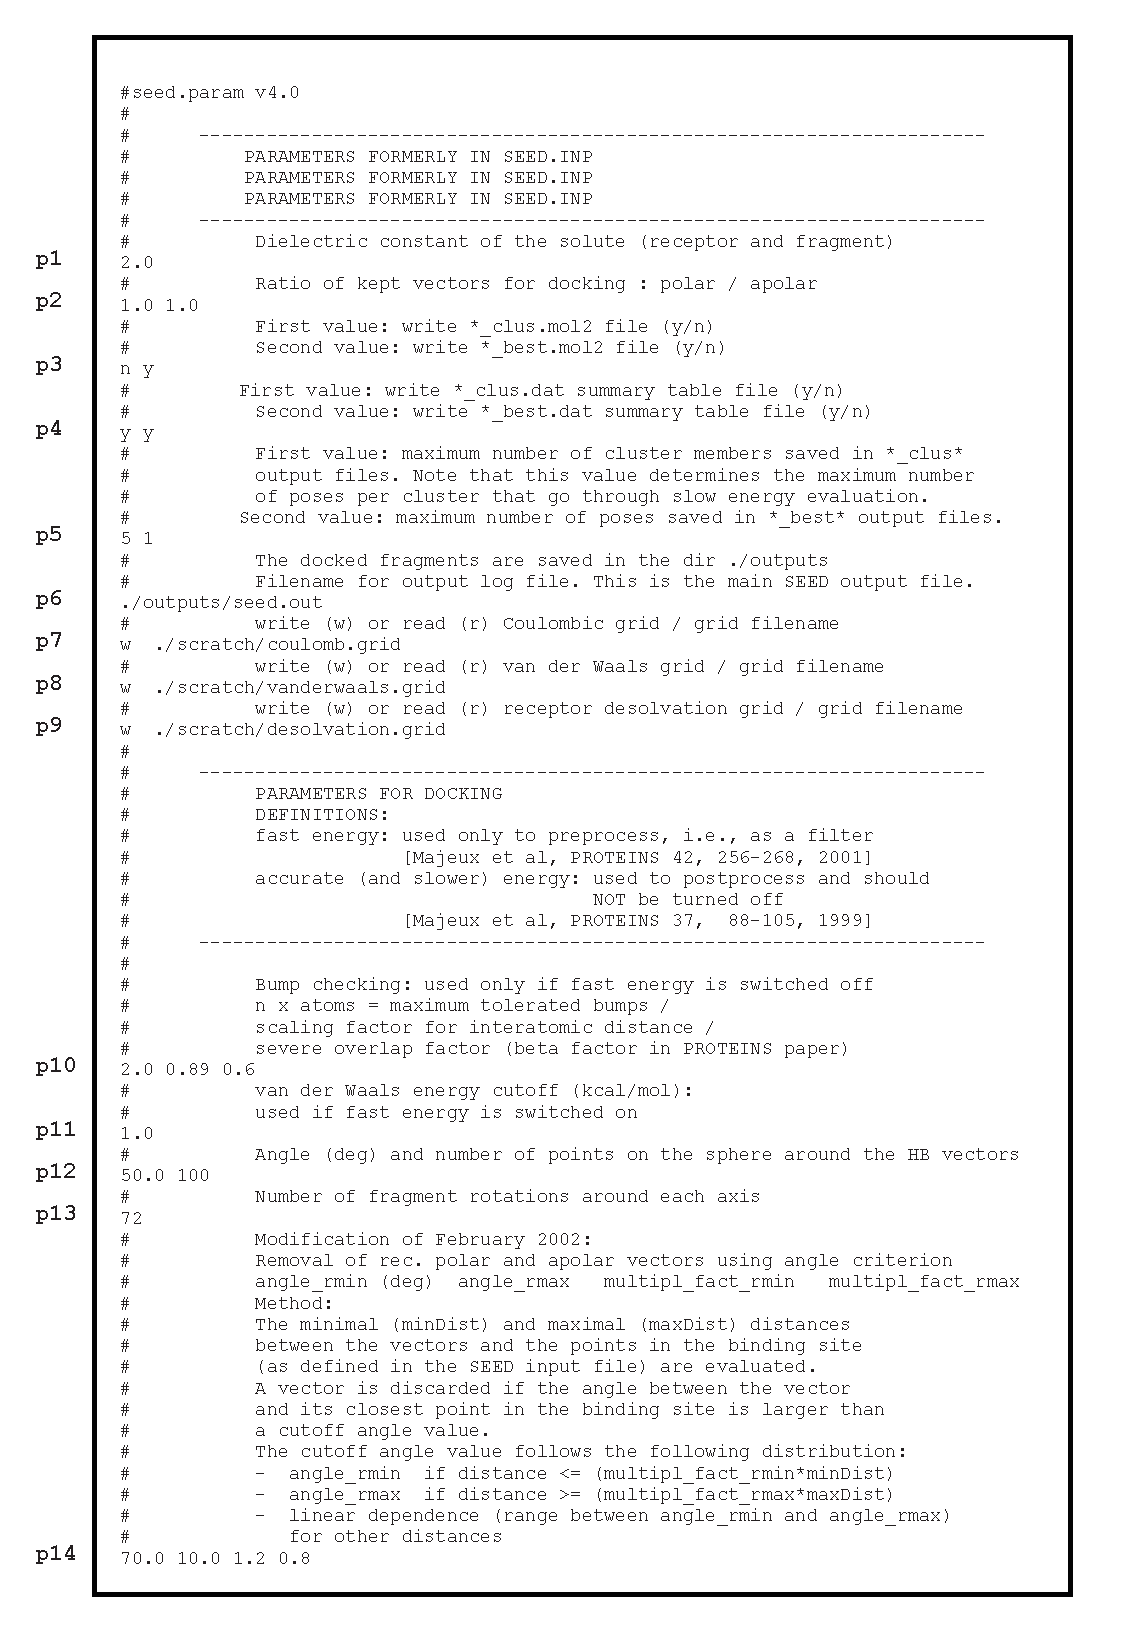
\includegraphics[width=1.0\textwidth,keepaspectratio]{data/par_doc1_final.pdf}}
  \caption*{\textit{Seed input file (\textbf{seed.par}) 1/4.}}
  %\vspace*{4in}
\end{figure}


% %\begin{figure}
% \vspace*{-1.7cm}
% \begin{center}
% 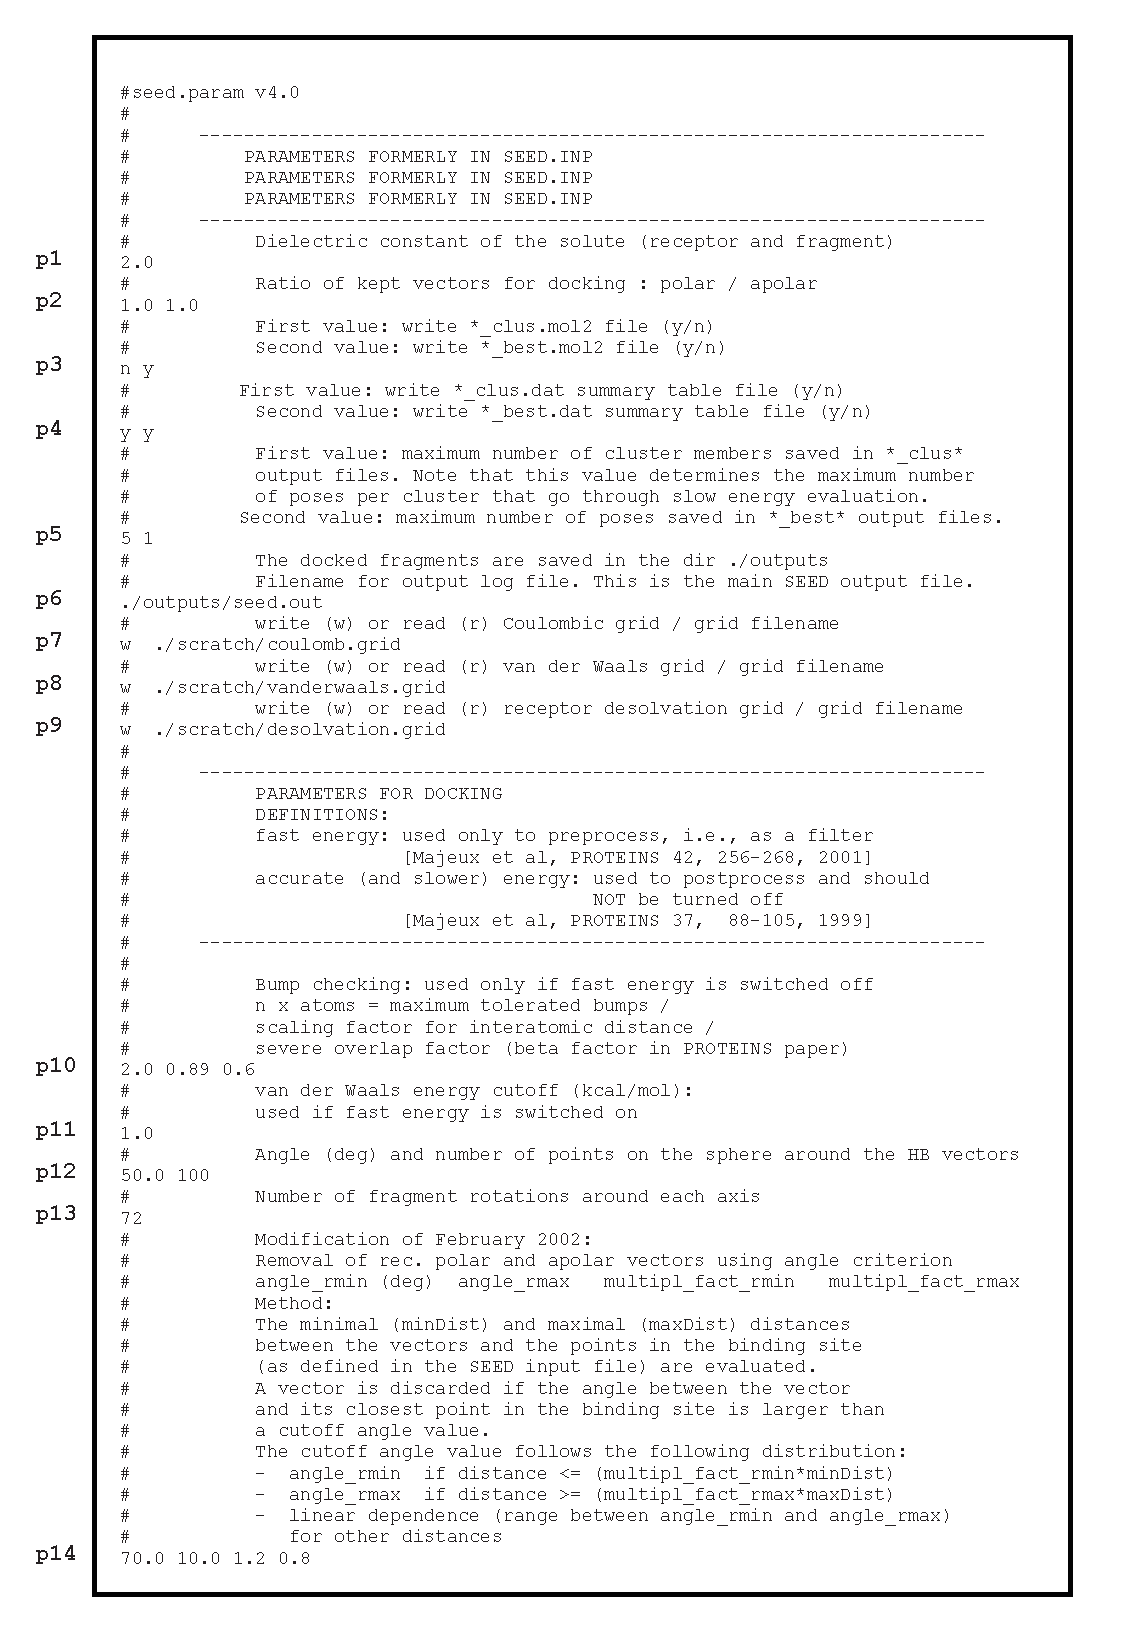
\includegraphics[scale=0.9]{data/par_doc1_final.pdf}
% \end{center}
% %\end{figure} 

%\newpage

\begin{figure}[p]
\vspace*{-1.2in}
  \centering
  \makebox[\textwidth][c]{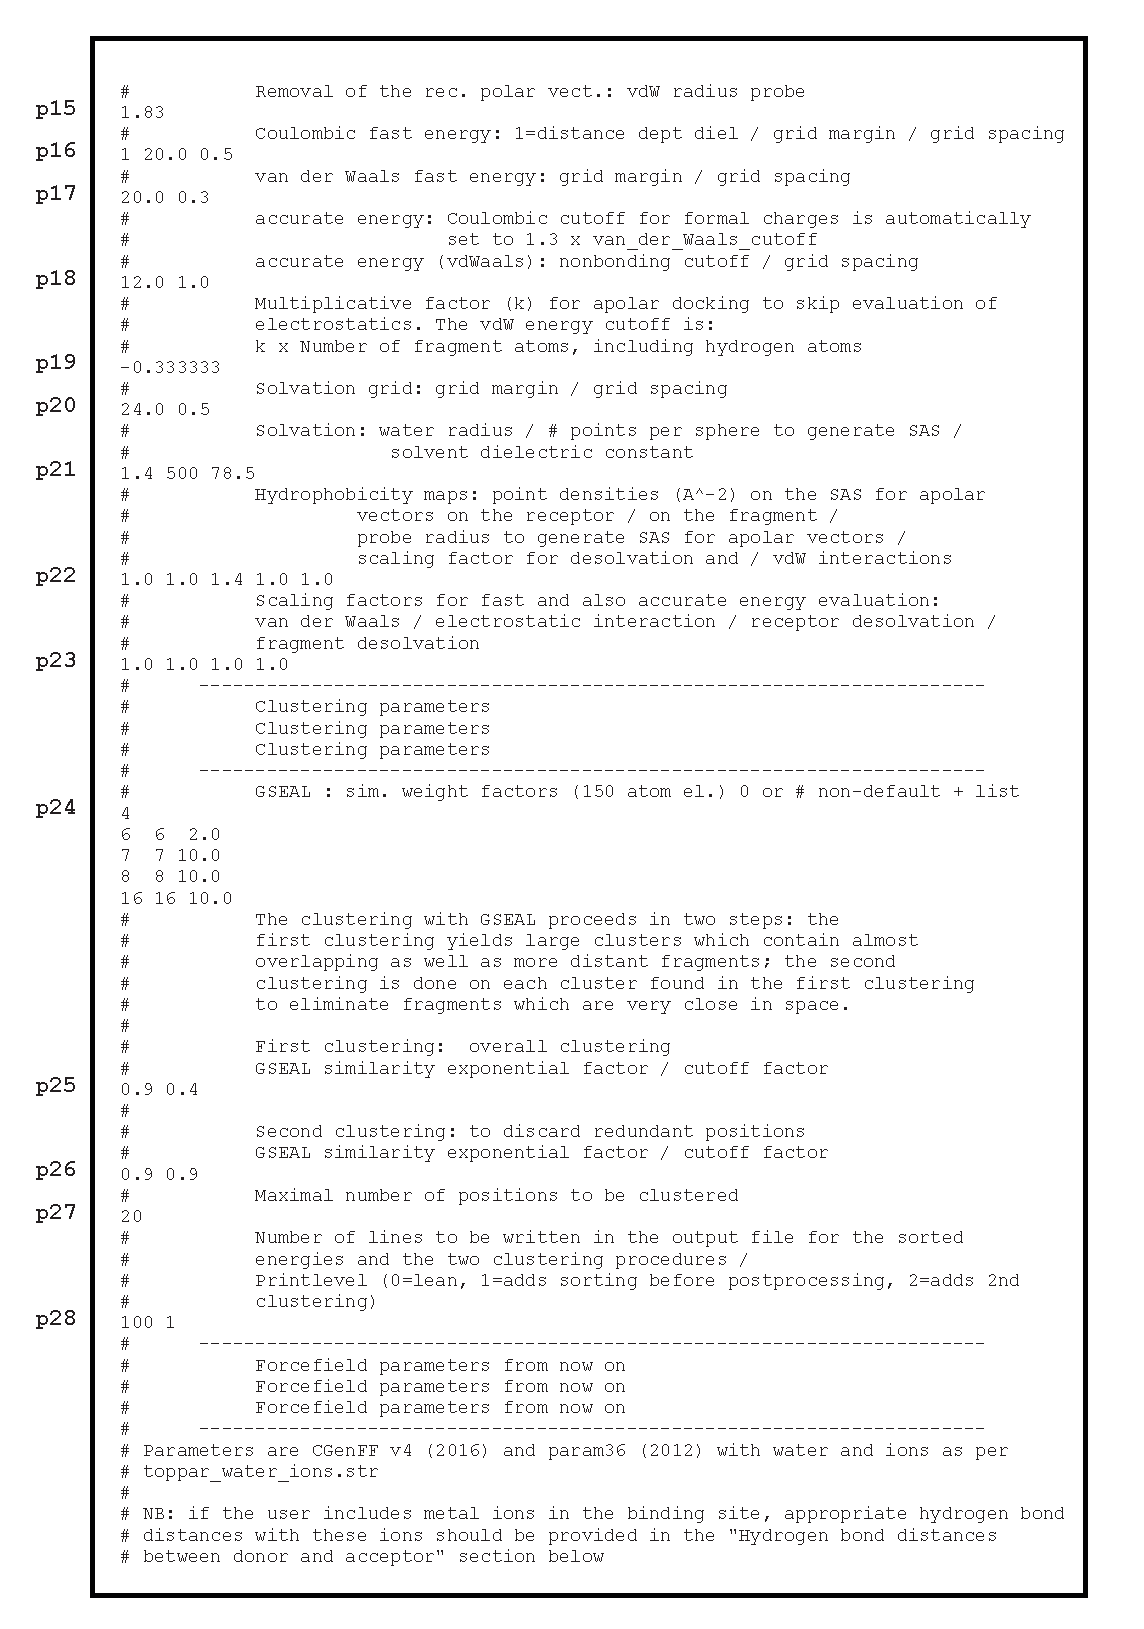
\includegraphics[width=1.0\textwidth,keepaspectratio]{data/par_doc2_final.pdf}}
  \caption*{\textit{Seed input file (\textbf{seed.par}) 2/4.}}
  %\vspace*{4in}
\end{figure}

% \begin{figure}
% \begin{center}
% \includegraphics[scale=0.9]{data/par2.pdf}
% \end{center}
% \end{figure} 

%\newpage

\begin{figure}[p]
\vspace*{-1.2in}
  \centering
  \makebox[\textwidth][c]{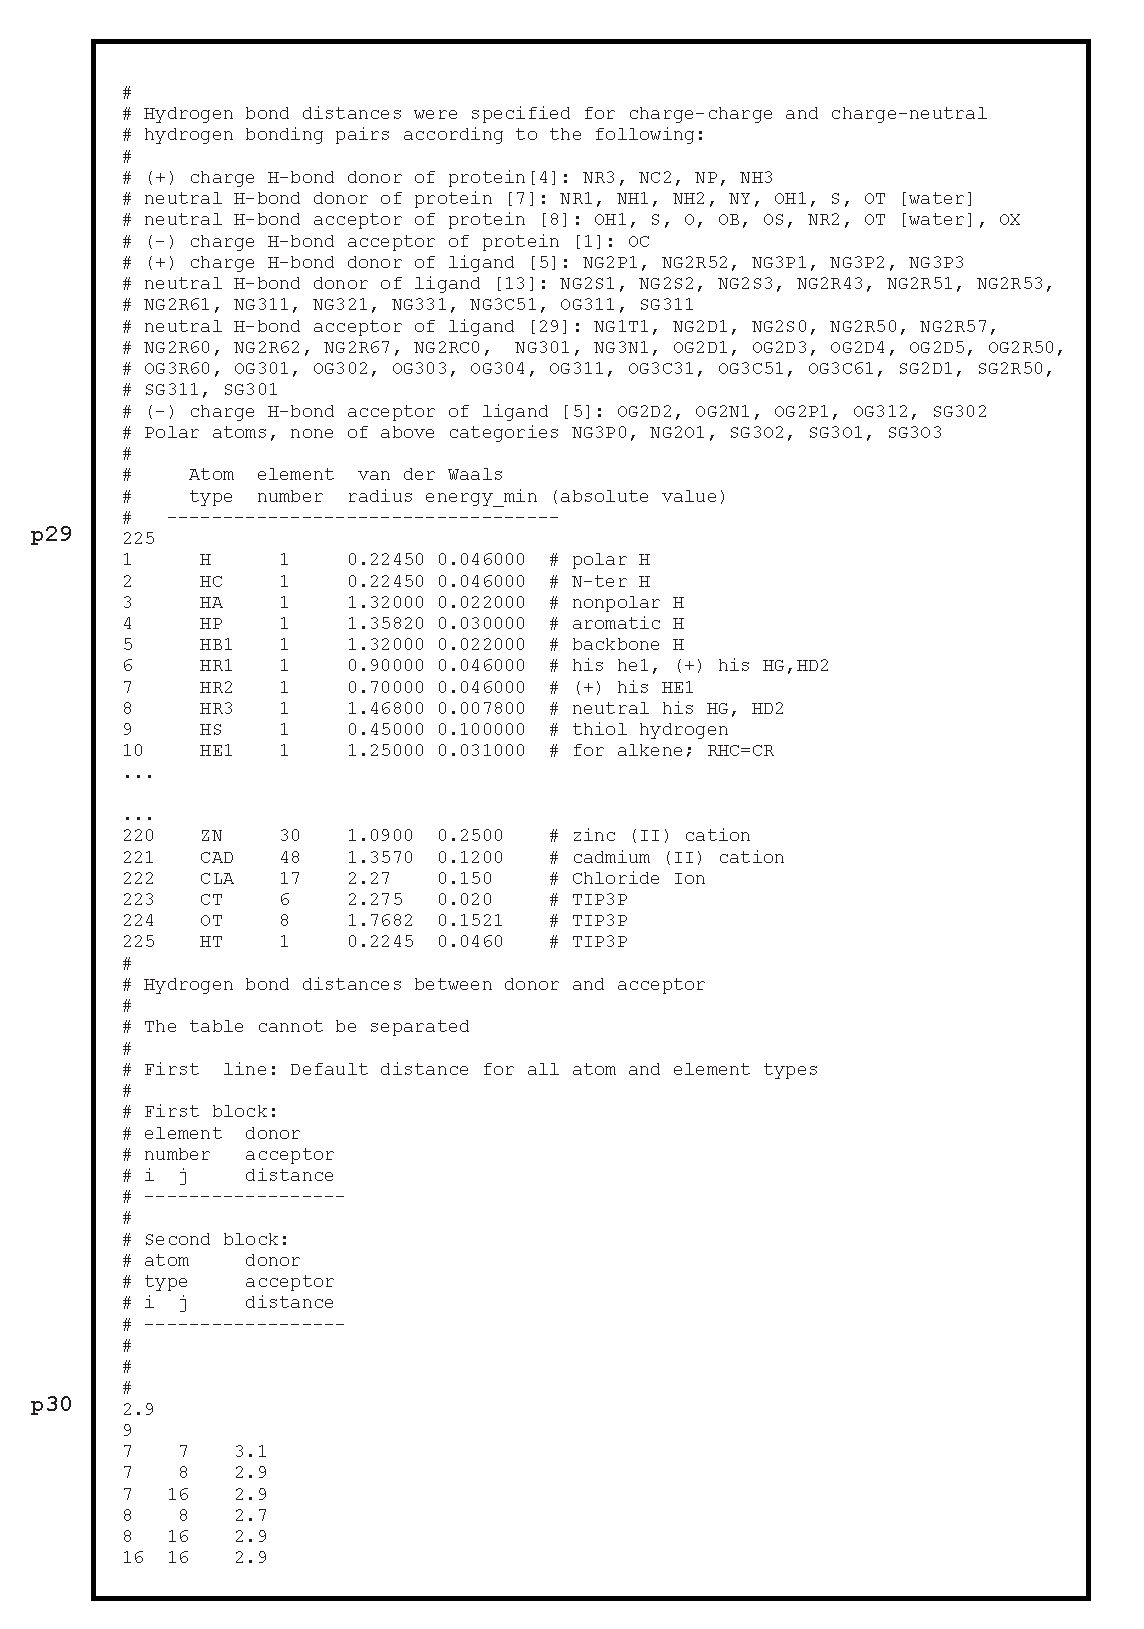
\includegraphics[width=1.0\textwidth,keepaspectratio]{data/par_doc3_final.pdf}}
  \caption*{\textit{Seed input file (\textbf{seed.par}) 3/4.}}
  %\vspace*{4in}
\end{figure}

% \begin{figure}
% \begin{center}
% \includegraphics[scale=0.9]{data/par3.pdf}
% \end{center}s
% \end{figure} 

%\newpage

\begin{figure}[p]
\vspace*{-1.2in}
  \centering
  \makebox[\textwidth][c]{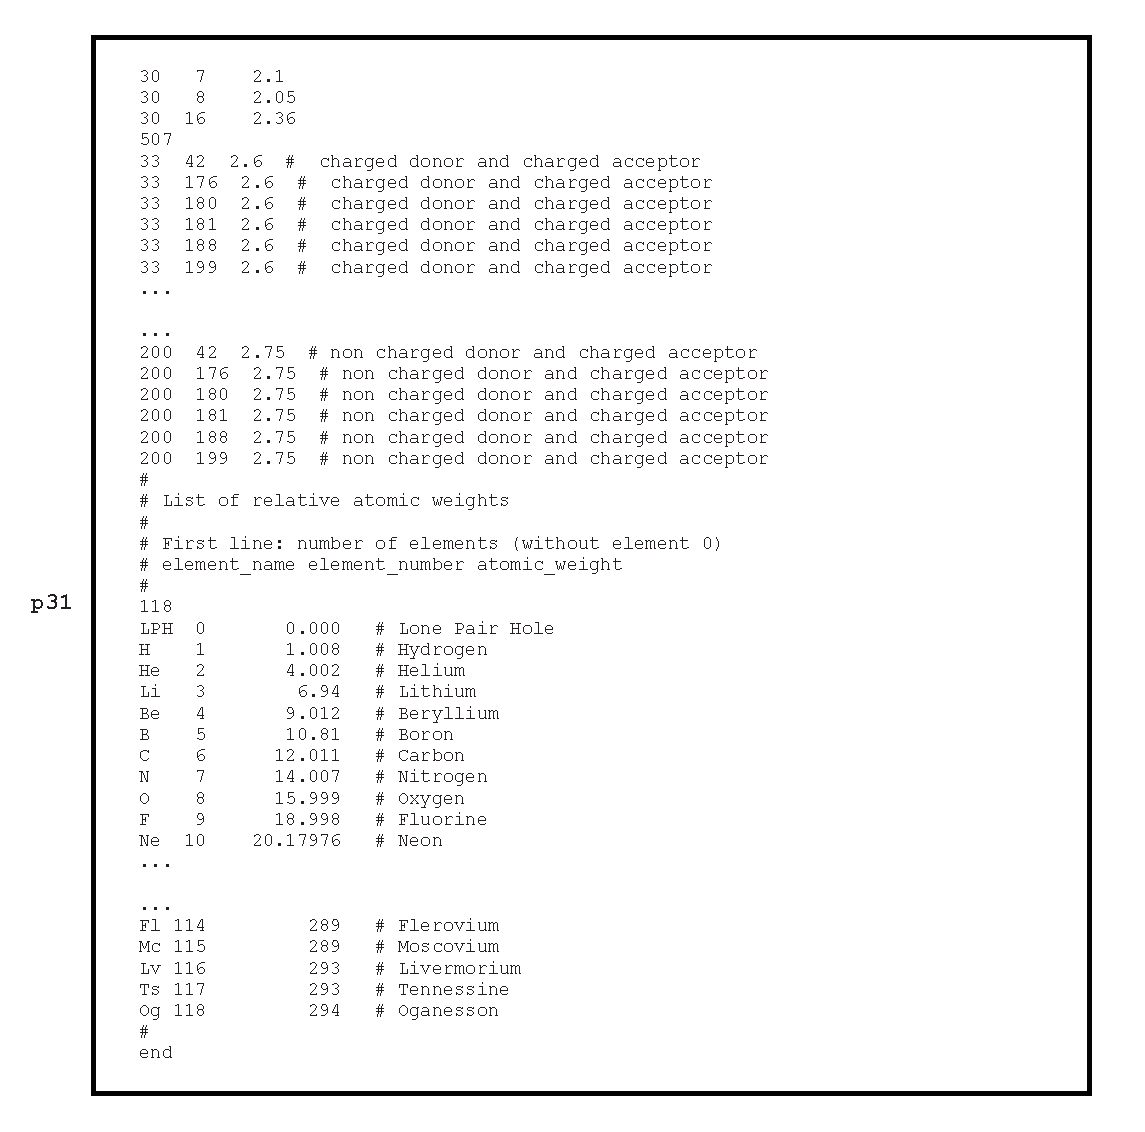
\includegraphics[width=1.0\textwidth,keepaspectratio]{data/par_doc4_final.pdf}}
  \caption*{\textit{Seed parameter file (\textbf{seed.par}) 4/4.}}
  %\vspace*{4in}
\end{figure}

%\newpage

\begin{comment}
\begin{figure}
%\begin{center}
\vspace*{-1in}
\centering
\makebox[\textwidth][c]{\includegraphics[scale=0.8]{data/ChangeLog_SEED3_3_1.ps}}
%\end{center}
\end{figure} 

\newpage

\begin{figure}
\begin{center}
\makebox[\textwidth][c]{\includegraphics[scale=0.8]{data/ChangeLog_SEED3_3_2.ps}}
\end{center}
\end{figure} 

\newpage

\begin{figure}
\begin{center}
\makebox[\textwidth][c]{\includegraphics[scale=0.8]{data/ChangeLog_SEED3_3_3.ps}}
\end{center}
\end{figure} 

\newpage

\begin{figure}
\begin{center}
\makebox[\textwidth][c]{\includegraphics[scale=0.8]{data/ChangeLog_SEED3_3_5.ps}}
\end{center}
\end{figure} 

\newpage

\begin{figure}
\begin{center}
\makebox[\textwidth][c]{\includegraphics[scale=0.8]{data/ChangeLog_SEED3_3_6.ps}}
\end{center}
\end{figure}
\end{comment}

\end{document}
